\documentclass[12pt, a4paper]{article}
\usepackage[margin=1in]{geometry}

\usepackage[english]{babel}
\usepackage{amsmath}
\usepackage{amssymb}
\usepackage{graphicx}
\usepackage[colorlinks=true, allcolors=blue]{hyperref}
\usepackage{fontawesome}
\usepackage{tikz}
\usepackage{longtable}

\usepackage{cmbright}
% \renewcommand*\familydefault{\sfdefault}
\usepackage[OT1]{fontenc}

\title{
	Conformalized
	%Quantile
	Zero-Shot Forecasting
}
\author{Nikolaos Kontogeorgis}
\date{}
\begin{document}
\maketitle

\begin{abstract}
	% Large-scale pre-trained
	Time Series Foundation Models (TSFMs) have transformed the time series prediction landscape by enabling zero-shot forecasting with accurate point predictions and even native uncertainty quantification via quantile outputs. By rigorously evaluating against post-hoc conformal prediction (CP) calibration, we show that these quantile outputs can be poorly calibrated. We provide a standardized application of and comparison between CP variants in this setting, and demonstrate that they can significantly improve coverage over native TSFM quantiles.
\end{abstract}

\section{Introduction}
Time series forecasting is a critical task across various domains, including finance, healthcare, weather prediction, and supply chain management, where accurate future predictions drive essential decision-making. Traditionally, forecasting has relied on statistical methods such as ARIMA or Exponential Smoothing, as well as machine learning approaches like Gradient Boosting or recurrent neural networks (RNNs) trained specifically on individual datasets. While effective for well-defined problems, these traditional methods often struggle to generalize across diverse domains and require extensive dataset-specific tuning.

Recently, the paradigm has shifted with the introduction of Time Series Foundation Models (TSFMs). Inspired by the success of large language models, TSFMs are pre-trained on massive, diverse datasets, enabling them to capture universal temporal patterns. Models such as TimesFM, Chronos, and FlowState have demonstrated undoubted point prediction performance, often achieving state-of-the-art results in zero-shot settings without the need for task-specific fine-tuning.

However, in many real-world applications, point predictions are insufficient. Uncertainty quantification (UQ) is often useful or even strictly required to assess the reliability of a forecast and mitigate risks. Even though most modern TSFMs now offer native UQ capabilities---such as outputting predictive distributions or utilizing quantile regression---these estimates generally come with no formal statistical guarantees. They can be overly confident or poorly calibrated, especially when applied to unseen data distributions in a zero-shot manner.

To bridge this gap, Conformal Prediction (CP) offers a powerful, distribution-free framework for rigorous uncertainty quantification. By constructing prediction intervals that are guaranteed to contain the true future values with a user-specified probability, CP provides the missing reliability to TSFM forecasts. In this work, we explore the integration of time-series-specific conformal prediction methods with state-of-the-art TSFMs, aiming to combine the exceptional zero-shot predictive power of foundation models with the robust, mathematically sound coverage guarantees of conformal inference.

\section{Background and Related Work}

\subsection{Time Series Foundation Models}
The paradigm of foundation models, which has revolutionized natural language processing and computer vision, is increasingly being adapted for time series analysis. Time Series Foundation Models (TSFMs) are typically pre-trained on massive, diverse datasets, allowing them to capture universal temporal patterns and enabling zero-shot or few-shot inference on unseen datasets. These models can be broadly categorized based on their architectural choices and representation strategies.

\paragraph{Patch-based and Generic Transformers}
Early efforts to scale time series forecasting demonstrated that segmenting time series into sub-sequence patches significantly improves the capability of Transformers to capture local semantics and long-term dependencies. A notable milestone in this direction is PatchTST \cite{patchtst}, which leverages channel-independent processing and patching to establish a strong baseline for subsequent foundation models.

\paragraph{Decoder-Only and Language-Model-Based Models}
Drawing inspiration from large language models, several TSFMs employ decoder-only architectures, often treating time series values as sequences of tokens or patches. TimesFM \cite{timesfm} (and its later iterations like TimesFM-2.5) is a decoder-only foundation model explicitly designed for time series forecasting that processes patches of data to maintain competitive inference speed and accuracy. Chronos-2 \cite{chronos2} is a prominent example that learns the ``language'' of time series by tokenizing continuous values and training an autoregressive language model, demonstrating strong zero-shot capabilities for universal forecasting. Toto-2 \cite{toto2} similarly scales autoregressive time series forecasting to massive datasets, highlighting the benefits of scaling laws in the time series domain.

\paragraph{Enhanced In-Context Learning and Continuous Representations}
While transformer-based and autoregressive token models are powerful, alternative architectures aim to improve forecasting by utilizing continuous representations, recurrent state-tracking, or state space models. Unlike most TSFMs that rely on transformers, TiRex \cite{tirex} leverages xLSTM---an enhanced Long Short-Term Memory network---to retain strict recurrent state-tracking, which proves critical for robust in-context learning and long-horizon zero-shot forecasting. Conversely, FlowState \cite{flowstate} departs from discrete patch or token processing by utilizing a state space model (SSM) based encoder coupled with a functional basis decoder. This unique architectural choice enables continuous-time modeling and dynamic time-scale adjustments, providing an inherently sampling-rate invariant formulation that generalizes effectively across frequencies without needing to memorize patterns at every scale. Finally, returning to the transformer paradigm, Timer-S1 \cite{timer-s1} pushes the boundary of sheer scale, introducing a billion-scale time series foundation model that employs serial scaling techniques to handle massive context lengths and complex temporal relationships.

\paragraph{Multi-step Forecasting}
It is important to note that current Time Series Foundation Models mostly perform direct multi-step forecasting. Unlike traditional autoregressive models that predict one step at a time, TSFMs take a historical context window as input and directly output a sequence of future predictions over a specified forecasting horizon.

\subsection{Conformal Prediction}
% \subsubsection{The Conformal Prediction Framework}
Conformal prediction (CP)~\cite{vovk2005algorithmic} is a versatile, distribution-free framework for uncertainty quantification. Given a user-specified error rate or \textit{miscoverage rate} \(\alpha \in (0,1)\), CP constructs prediction intervals (or sets) that are mathematically guaranteed to contain the true test response with probability at least \(1-\alpha\). This theoretical guarantee, known as \textit{marginal coverage}, holds regardless of the underlying data distribution or the chosen base predictive model, provided that the data points are exchangeable (i.e., the joint probability distribution is invariant to permutations of the indices).

The calibration process in the standard split CP setup proceeds as follows. First, the available data is divided into a training set and a disjoint \textit{calibration set}. A base machine learning model is trained on the training set. Then, a heuristic notion of uncertainty is encapsulated into a \textit{non-conformity score}, which measures how unusual a new observation is relative to the model's predictions. These scores are computed for all instances in the calibration set. By calculating the empirical \(\frac{\lceil (n + 1)(1 - \alpha) \rceil}{n}\) quantile of these calibration non-conformity scores (where \(n\) is the size of the calibration set), CP determines a critical threshold. Finally, for any new test point, the prediction interval is constructed by including all possible target values whose non-conformity score falls below this calibrated threshold. This elegantly simple procedure calibrates the output of any base model into valid, theoretically sound prediction intervals without making strong distributional assumptions.

\subsubsection{Methods for Time Series Data}
Applying standard split CP to time series data presents significant theoretical and practical challenges. The primary obstacle is the violation of the exchangeability assumption. Time series data exhibit temporal dependencies, autocorrelations, and non-stationarity (such as concept drift, seasonality, and varying volatility). Consequently, the non-conformity scores evaluated on past data may not reliably represent the distribution of scores for future observations. When standard CP is applied naively to time series, it often results in severe under-coverage or unnecessarily wide, uninformative prediction intervals. Thus, specialized adaptations of the CP framework are required to dynamically adjust to changing environments and shifting distributions.

To address the lack of exchangeability, a growing body of literature has developed conformal prediction methods specifically tailored for time series data. These methods can be broadly categorized into the following groups:

\paragraph{Ensemble and Other Model-Conditional Techniques}
Ensemble methods discard the exchangeability assumption directly by utilizing robust ensemble techniques. EnbPI (Ensemble prediction intervals)~\cite{enbpi-1} introduced this family of methods by constructing sequential prediction intervals around bootstrap ensemble estimators without requiring data exchangeability, assuming instead that the errors are strongly mixing. EnCQR~\cite{encqr} extends this idea to quantile regression, constructing prediction intervals around ensemble quantile regression models. Both methods are particularly well-suited for time series data, where temporal dependencies often violate the exchangeability assumption. These approaches however require training multiple models on subsets of data, which can be computationally intensive and does not align well with the concept of foundation models that are designed for zero-shot inference.

\paragraph{Adaptive and Online Conformal Inference}
One prominent model-agnostic approach is to adapt the target error rate or the interval width iteratively based on past coverage performance. If recent intervals have been under-covering the true values, the algorithm widens the intervals for subsequent predictions; conversely, it narrows them if over-coverage is detected. Adaptive Conformal Inference (ACI) \cite{aci} and its variations AgACI~\cite{agaci} and DtACI~\cite{dtaci} follow this principle. More recent works have formulated this adaptation as a dynamical system control problem, introducing Conformal PID Control \cite{c-pid} and Neural Conformal Control \cite{ncc} to achieve robust sequential coverage.

\paragraph{Handling Covariate Shift and Change Points}
A distinct line of research focuses on adapting conformal prediction when the underlying distribution exhibits explicit shifts or abrupt structural changes. Early work modified the CP procedure by reweighting non-conformity scores to account for covariate shift \cite{weighted-cp}. Later, general theoretical frameworks were developed to understand conformal prediction beyond exchangeability \cite{nex-cp}, quantifying the coverage gap induced by such distribution shifts. When facing highly non-stationary environments, specialized methods have also been introduced to maintain valid coverage in the presence of abrupt change points \cite{cptc}.

\paragraph{Robust Ensemble and Sequential Methods}
Other methods relax the exchangeability assumption directly by utilizing robust ensemble techniques and sequential calibration. For instance, EnbPI (Ensemble prediction intervals) \cite{enbpi-1} constructs sequential prediction intervals around bootstrap ensemble estimators without requiring data exchangeability, assuming instead that the errors are strongly mixing. Building upon this, Sequential Predictive Conformal Inference (SPCI) \cite{spci} leverages sequential non-conformity scores and updates the calibration set dynamically to better capture local temporal dynamics.

\paragraph{Conformalized Quantile Regression and Temporal Adjustments}
Combining conformal prediction with quantile regression allows the construction of intervals that naturally adapt their width to heteroscedasticity. Methods like Ensemble Conformalized Quantile Regression (Ensemble CQR) \cite{encqr} apply this to probabilistic time series forecasting. Additionally, adjusting non-conformity scores through Temporal Quantile Adjustments \cite{tqa} helps in capturing varying temporal uncertainties, resulting in tighter and more reliable intervals.

\subsubsection{Multi-step Forecasting}
While many methods focus on one-step-ahead forecasting, extending CP to multi-step horizons requires capturing joint distributions over future time steps. CF-RNN~\cite{confrnn} addresses the exchangeability collapse by dividing the data into training/calibration/test splits across timeseries rather than across the time axis. D Copula Conformal Prediction \cite{copulacpts} utilizes copulas to model the dependencies among future steps for coherent multi-step intervals. Advanced perspectives such as Bellman Conformal Inference \cite{bellman-ci} connect conformal prediction to dynamic programming and reinforcement learning to calibrate intervals for sequential decision-making. Multi-dimensional forecasting challenges are addressed by Flow-based Conformal Prediction \cite{flow-cp}, employing classifier-free guidance to construct tighter prediction sets. Finally, recent work has also explored integrating conformal prediction directly into specialized neural architectures, such as modern Hopfield networks \cite{hop-cpt}, to leverage their continuous state representations for more robust uncertainty quantification.

\subsection{Conformal Prediction for Time Series Foundation Models}
The intersection of Conformal Prediction (CP) and Time Series Foundation Models (TSFMs) is an emerging and highly promising area of research. By leveraging the strong zero-shot predictive capabilities of TSFMs, researchers can apply post-hoc uncertainty quantification methods like CP more effectively. The most direct precursor to our work is \cite{ts-genai-cp}, where authors demonstrate that the zero-shot nature of FMs allows a larger proportion of available historical data to be allocated strictly for calibration rather than model training. This results in more stable and reliable conformalized prediction intervals, particularly in data-constrained scenarios where traditional statistical or machine learning models struggle due to limited training samples. However, this work only includes standard split CP as the method of choice instead of more advanced methods that are designed to handle the specific challenges of time series data, and its dataset choice is limited.

Even if previously unexplored, the integration of time series-specific CP methods with TSFMs is a natural next step. For example, adaptive conformal inference techniques could be applied to the outputs of TSFMs to dynamically adjust prediction intervals in response to detected distribution shifts or temporal dynamics. Similarly, methods designed to handle covariate shift and change points could be particularly beneficial when applied to the forecasts of TSFMs, which may encounter varying patterns across different datasets or time periods. One exception is ensemble-based methods like EnbPI and EnCQR, because their demand of training multiple models on subsets of data is inherently in contrast with the concept of TSFMs.

% Furthermore, CP has been successfully integrated with TSFMs for tasks beyond standard forecasting, such as anomaly detection. Work by Gil et al. \cite{w1-acas} proposes an adaptive conformal anomaly detection method that utilizes pre-trained TSFMs without the need for additional fine-tuning. By employing weighted quantile conformal prediction bounds and adaptively learning weighting parameters from past predictions, their method maintains stable false alarm control under distribution shifts while providing interpretable anomaly scores.

These integrations highlight the significant potential of combining the representational power of foundation models with the rigorous, distribution-free statistical guarantees provided by conformal prediction.

\section{Experimental Setup}
\subsection{TSFMs}
To rigorously evaluate the integration of conformal prediction with modern foundation models, we select a shortlist of four state-of-the-art Time Series Foundation Models (TSFMs): \textbf{Chronos-2}~\cite{chronos2}, \textbf{TimesFM}~\cite{timesfm} (specifically TimesFM 2.5), \textbf{TiRex}~\cite{tirex}, and \textbf{FlowState}~\cite{flowstate}. These models were chosen based on four primary criteria: (1) high public adoption and community usage, (2) ease of use and API integration, (3) strong performance on prominent large-scale benchmarks such as GIFT-Eval~\cite{gift-eval}, TIME~\cite{time}, and FEV~\cite{fev-bench}, and (4) architectural diversity.

Architecturally, the shortlisted models represent distinct paradigms:
\begin{itemize}
	\item \textbf{TimesFM} and \textbf{Chronos-2} are popular transformer-based designs representing decoder-only and encoder-only designs respectively.
	\item \textbf{TiRex} represents an LSTM-based paradigm, utilizing the advanced xLSTM architecture to achieve enhanced recurrent state-tracking and in-context learning.
	\item \textbf{FlowState} represents a state-space model (SSM) based architecture, employing a continuous-time SSM encoder with a functional basis decoder.
\end{itemize}
By choosing models spanning transformer, recurrent (LSTM), and state-space (SSM) designs, we can evaluate how post-hoc conformal prediction calibrates forecasts across fundamentally different underlying architectures.

\subsection{Datasets}
To evaluate the robustness, generalization, and calibration of conformalized TSFMs, we identify four major time-series meta-datasets: \textbf{GIFT-Eval}~\cite{gift-eval}, \textbf{TIME}~\cite{time}, \textbf{BOOM}~\cite{toto}, and \textbf{FEV}~\cite{fev-bench}.

\begin{itemize}
	\item \textbf{GIFT-Eval}~\cite{gift-eval} is currently the most widespread benchmark for general time series forecasting. However, some of the modern TSFMs include subsets of its constituent datasets in their pre-training corpora, meaning evaluations on it are not truly zero-shot.
	\item \textbf{TIME}~\cite{time} directly addresses this pre-training leakage by introducing novel, unseen-before temporal datasets specifically selected to guarantee genuine zero-shot evaluation.
	\item \textbf{BOOM}~\cite{toto} is a specialized benchmark that focuses on specific industrial subdomains, most notably IT observability and systems monitoring (e.g., CPU, memory, and network telemetry).
\end{itemize}

Ultimately, we select the \textbf{FEV} (Forecasting Evaluation and Verification) benchmark~\cite{fev-bench} for our main evaluations. We chose FEV for several reasons: first, it is highly comprehensive, incorporating diverse datasets from both GIFT-Eval and BOOM, among other sources; second, it provides a well-defined small subset of representative tasks (\textbf{FEV-bench mini}, which we selected for our final experiments) that accurately represents the complexity of the full benchmark while remaining computationally tractable; third, we found the FEV framework and task layout to be significantly better documented and more straightforward to use and integrate into our evaluation pipeline compared to other meta-datasets.

\subsection{Conformal Prediction Methods}
We evaluate a representative set of conformal prediction (CP) methods that are well-suited for sequential time-series forecasting. These methods are post-hoc calibrators that take point forecasts and predictive distributions produced by TSFMs and generate mathematically sound prediction intervals. The evaluated methods are categorized as follows:

\begin{itemize}
	\item \textbf{Naive Split CP}~\cite{papadopoulos2002, vovk2005algorithmic}: A standard, static baseline that assumes exchangeability of nonconformity scores and does not perform online updates.
	\item \textbf{Weighted CP}~\cite{weighted-cp}: A baseline that uses decaying geometric weights over past nonconformity scores to prioritize recent observations, offering valid coverage guarantees under certain non-exchangeable distribution shifts.
	\item \textbf{Trailing Window}~\cite{dss}: A simple rolling-quantile method that computes empirical quantiles over a sliding window of the most recent scores without explicit error-rate tracking.
	\item \textbf{Adaptive Conformal Inference (ACI)}~\cite{aci}: An online method that dynamically updates the target miscoverage rate \(\alpha_t\) at each step based on whether the previous forecast fell within the prediction interval.
	\item \textbf{AgACI}~\cite{agaci} and \textbf{DtACI}~\cite{dtaci}: Robust expert-ensemble extensions of ACI that self-tune the step-size parameter \(\gamma\) using online learning algorithms (such as AdaHedge and exponential weights) to handle arbitrary distribution shifts.
	\item \textbf{Conformal PID Control (PID)}~\cite{c-pid}: Formulates online quantile tracking as a feedback control system, utilizing proportional-integral-derivative control to achieve robust, long-run coverage guarantees with minimal interval oscillation.
	\item \textbf{Autocorrelated Multi-step Conformal Prediction (AcMCP)}~\cite{acmcp}: An asymmetric, multi-step online calibration method that models the lag-\((h-1)\) autocorrelation structure inherent in multi-step forecast errors using a moving average and ordinary least squares scorecaster, optimizing interval width and coverage tracking.
\end{itemize}

\paragraph{Adaptation to Multi-step Forecasting}
Because Time Series Foundation Models perform direct multi-step forecasting---outputting a sequence of future predictions over a horizon \(H\) (i.e., \(\hat{y}_{t+1}, \dots, \hat{y}_{t+H}\)) rather than single-step predictions---traditional one-step conformal prediction algorithms (such as ACI, PID, or Split CP) must be adapted. We employ a \textit{step-independent marginal calibration} strategy. For a forecasting horizon \(H\), we instantiate \(H\) independent conformal calibrators, each dedicated to a specific look-ahead step \(h \in \{1, \dots, H\}\).

During calibration, nonconformity scores are computed and tracked separately for each horizon step. For these adapted methods, the control variables and interval adjustments are updated independently for each step \(h\), based solely on the historical coverage performance of that specific horizon. This step-wise marginal calibration targets nominal coverage pointwise across all future horizons and naturally accommodates the characteristic increase in predictive uncertainty over longer look-ahead steps. To evaluate the benefit of this structure, we compare it against a \textit{single-step baseline} mode, where all horizon steps are flattened into a single temporal stream, ignoring horizon-specific temporal structures.

Importantly, \textbf{AcMCP} is inherently a multi-step forecasting calibration method by design. Unlike the adapted methods which treat horizons as independent calibration tasks, AcMCP recursively models the lag-\((h-1)\) autocorrelation structure across future steps using a cross-horizon error forecasting model. Consequently, AcMCP does not require post-hoc multi-step adaptation in the same way as other methods, as multi-step cross-horizon dependencies are natively integrated into its error tracking equations.

\paragraph{Nonconformity Scores}
Rather than relying solely on standard residuals, we consider the complete spectrum of eleven physical, scaled, stateful, and quantile-grid nonconformity scores supported by our conformal evaluation pipeline:

\begin{itemize}
	\item \textbf{Standard Absolute Residuals (\texttt{abs})}: The absolute point-forecast error, \(s_t = |y_t - \hat{y}_t|\). This serves as the standard symmetric baseline, inverting to \([\hat{y}_t - q, \, \hat{y}_t + q]\).
	\item \textbf{Squared Residuals (\texttt{squared})}~\cite{lei2018distribution}: The squared point-forecast error, \(s_t = (y_t - \hat{y}_t)^2\). It penalizes outliers quadratically, inverting to the symmetric interval \([\hat{y}_t - \sqrt{\max(q, 0)}, \, \hat{y}_t + \sqrt{\max(q, 0)}]\).
	\item \textbf{Signed Residuals (\texttt{signed})}~\cite{lei2018distribution}: The signed point-forecast error, \(s_t = y_t - \hat{y}_t\). This score forces asymmetric calibration by constructing independent lower and upper bounds, inverting to \([\hat{y}_t - q_{lo}, \, \hat{y}_t + q_{up}]\).
	\item \textbf{IQR-Scaled Residuals (\texttt{iqr\_scaled})}~\cite{lei2018distribution}: A locally adaptive score where the absolute residual is normalized by the model's native quantile interval width, \(s_t = |y_t - \hat{y}_t| / \max(q_{high, t} - q_{low, t}, \epsilon)\). It enables prediction intervals to dynamically expand or shrink according to the foundation model's in-context uncertainty, inverting to \([\hat{y}_t - q(q_{high, t} - q_{low, t}), \, \hat{y}_t + q(q_{high, t} - q_{low, t})]\).
	\item \textbf{MAD-Scaled Residuals (\texttt{mad\_scaled})}~\cite{lei2018distribution}: Normalizes the residual by a robust estimate of local residual scale based on the Median Absolute Deviation (MAD), \(s_t = |y_t - \hat{y}_t| / \max(\rho_{mad, h}, \epsilon)\), where \(\rho_{mad, h} = 1.4826 \times \text{MAD}(\{y_i - \hat{y}_i\}_{i \in \text{cal}})\) is computed across the calibration set for each horizon step \(h\).
	\item \textbf{Conformalized Quantile Regression (\texttt{cqr})}~\cite{cqr}: The canonical CQR score, \(s_t = \max(q_{low, t} - y_t, \, y_t - q_{high, t})\). It directly calibrates the native lower and upper boundaries of the model's quantiles, inverting to \([q_{low, t} - q, \, q_{high, t} + q]\).
	\item \textbf{Scaled CQR (\texttt{scaled\_cqr})}~\cite{cqr}: Extends CQR by scaling the lower and upper violations separately using their respective robust calibration tail scales: \(s_t = \max((q_{low, t} - y_t)/\sigma_{lo, h}, \, (y_t - q_{high, t})/\sigma_{hi, h})\), inverting to \([q_{low, t} - q\sigma_{lo, h}, \, q_{high, t} + q\sigma_{hi, h}]\).
	\item \textbf{Pinball-CRPS Like (\texttt{distributional})}~\cite{gneiting-raftery, zamo-naveau}: The excess mean-pinball loss score evaluated over all \(K\) predicted quantile levels: \(s_t = S(y_t, \hat{F}_t) - \min_z S(z, \hat{F}_t)\), where \(S(y, \hat{F}_t) = \frac{1}{K}\sum_{k=1}^K \rho_{\tau_k}(y - q_{\tau_k, t})\) is the mean pinball loss. This uses the entire predicted quantile grid to calibrate a distributional-native interval, inverted through convex root-finding over the continuous pinball objective function.
	\item \textbf{CDF Tail (\texttt{cdf\_tail})}: A distribution-native score measuring the central-band probability integral transform (PIT) violation: \(s_t = \max(\alpha/2 - \hat{F}_t(y_t), \, \hat{F}_t(y_t) - (1 - \alpha/2), \, 0)\), where the cumulative distribution function \(\hat{F}_t(y)\) is estimated by monotonicized piecewise-linear interpolation over the predicted quantile grid. Inversion is solved directly on the probability scale as \([Q_t(\max(0, \alpha/2 - q)), \, Q_t(\min(1, 1 - \alpha/2 + q))]\).
	\item \textbf{Log-Scaled Residuals (\texttt{log})}~\cite{hyndman-fpp}: Formulated for multiplicative-error regimes, \(s_t = |\log(y_t + \epsilon) - \log(\hat{y}_t + \epsilon)|\), inverting to \([\exp(\log(\hat{y}_t + \epsilon) - q) - \epsilon, \, \exp(\log(\hat{y}_t + \epsilon) + q) - \epsilon]\). To prevent silent numerical errors, a domain preflight fallback automatically reverts to the \texttt{abs} score if nonpositive targets or predictions are detected on the calibration set.
	\item \textbf{Stateful Difference Residuals (\texttt{diff})}~\cite{chernozhukov-cqr}: A stateful, online nonconformity score that tracks the changes in sequential errors rather than their raw magnitude, \(s_t = |e_t - e_{t-1}|\), where \(e_t = y_t - \hat{y}_t\) represents the point-forecast residual. The resulting prediction interval is centered around the model's prediction shifted by the previous step's observed error: \([\hat{y}_t + e_{t-1} - q, \, \hat{y}_t + e_{t-1} + q]\).
\end{itemize}

\subsection{Experimental Variables and Controls} \label{subsec:controls}
To establish a rigorous, causal understanding of conformal calibration performance on pre-trained Time Series Foundation Models, we systematically control for and isolate the following experimental variables:

\begin{enumerate}
	\item \textbf{Conformal Prediction Method and Family}: We categorize our eight evaluated conformal methods into three structural families: (a) \textit{Static split methods} (SplitCP, WeightedCP) which establish global thresholds; (b) \textit{Adaptive online methods} (ACI, AgACI, DtACI, Conformal PID) which sequentially adjust thresholds in response to dynamic coverage errors; and (c) \textit{Time-series specific multi-step formulations} (AcMCP) which directly model cross-horizon error dependencies.

	\item \textbf{Autocorrelation and Horizon Adjustments}: For the online adaptive methods, we control for the calibration dimension by comparing our proposed \textit{step-independent marginal calibration} strategy (where an independent online controller tracks errors separately for each step \(h \in \{1, \dots, H\}\)) against a flattened \textit{single-step baseline} stream. This enables us to measure the empirical benefit of isolating horizon-specific temporal structures.

	\item \textbf{Nonconformity Score Formulation}: We isolate the effect of the uncertainty heuristic by evaluating eleven different nonconformity scores, spanning point-residual scales (\texttt{abs}, \texttt{squared}, \texttt{signed}, \texttt{log}, \texttt{diff}), adaptive boundary scaling (\texttt{iqr\_scaled}, \texttt{mad\_scaled}, \texttt{scaled\_cqr}), and complete quantile-grid probability models (\texttt{distributional}, \texttt{cdf\_tail}).

	\item \textbf{Model Architecture and Inductive Biases}: While pre-training datasets and scaling techniques differ across the evaluated foundation models, we evaluate across three fundamentally distinct architectural classes: decoder-only transformers (TimesFM), tokenized encoder-decoders (Chronos-2), LSTM-based state-trackers (TiRex), and continuous state-space models (FlowState). This allows us to observe how underlying inductive biases influence native in-context calibration.

	\item \textbf{Calibration Context and Covariate Shift}: We control for the source of the calibration data by comparing local sequential calibration (calibrating on the immediate chronological history of the target series) against cross-sectional calibration (calibrating across a pool of other series within the same meta-dataset). This isolates the impact of local non-stationarity and cross-series covariate shift.

	\item \textbf{Task Properties (Horizon, Domain, and Frequency)}: To evaluate the zero-shot generalization envelope of the calibrated forecasts, we run our experiments on diverse domains in the FEV benchmark. We control for target forecast horizons ranging from short-range (\(H=5\)) to ultra-long-range (\(H=288\)) steps, as well as multiple sampling frequencies (annual, daily, hourly, and weekly), and varying context lengths.
\end{enumerate}

\subsection{Representative Configuration Selection Criteria}
Due to the vast hyperparameter space spanning the cross-product of Time Series Foundation Models, conformal prediction methods, and nonconformity score types, a full exhaustive search across all possible combinations yields \(398\) unique configurations (as detailed in Appendix~\ref{sec:appendix_grid_search}). To present a clear, structured, and interpretable synthesis of results in the main text (Tables~\ref{tab:calibration_results_part1} and~\ref{tab:calibration_results_part2}), we selected a highly representative subset of nine configurations. This selection is governed by three primary criteria:

\begin{enumerate}
	\item \textbf{Systematic Representation of Method Families}: The selected configurations span all major taxonomic classes of conformal inference, including standard static baselines (SplitCP), distribution-shift-aware weighting (WeightedCP), heuristics without feedback (TrailingWindow), fully online adaptive frameworks (ACI, DtACI), and time-series-specific multi-step modeling (AcMCP).
	\item \textbf{Coverage of Nonconformity Score Families}: The configurations incorporate each of the main score categories: scale-free physical absolute residuals (\texttt{abs}), outlier-magnifying squared residuals (\texttt{squared}), asymmetric point-residuals (\texttt{signed}), locally scaled residuals (\texttt{iqr\_scaled}), quantile-boundary deviations (\texttt{cqr}), and grid-based distribution-native scores (\texttt{cdf\_tail}, \texttt{distributional}).
	\item \textbf{Delineation of Success Regimes and Failure Modes}: Rather than cherry-picking only optimal results, we select both high-performing calibrators (to show how to successfully close the calibration gap) and representative pathological failures. Specifically, we include TrailingWindow + Squared to represent undercoverage failures, and ACI + IQR-Scaled to represent the catastrophic runaway width explosion failure.
\end{enumerate}

To verify that these nine configurations are representative of the larger \(398\)-configuration search space, we perform a structured verification analysis:
\begin{itemize}
	\item \textbf{Distributional Coverage}: The selected successful methods (SplitCP + CDF-Tail, ACI + CDF-Tail, DtACI + CDF-Tail, and WeightedCP + Distributional) consistently represent the upper-bound envelope of achievable calibration. On the other hand, AcMCP + CQR illustrates the behavior of multi-step specific formulations, while the chosen failure cases represent the extreme boundaries of undercoverage (\(\approx 35\%\) coverage) and runaway width inflation (\(>10^{200}\) scaled width), ensuring the full performance distribution is spanned.
	\item \textbf{Score Efficiency Representation}: The selection highlights the clear superiority of grid-based scores (\texttt{cdf\_tail} and \texttt{distributional}) over traditional boundary-only or absolute residuals. Pairwise comparisons (e.g., DtACI + CDF-Tail vs. DtACI + Distributional) are retained to represent how different grid inversion strategies trade interval width efficiency for marginal coverage stability.
\end{itemize}
This structured subset enables us to conduct rigorous comparative analyses across fundamentally distinct theoretical frameworks while keeping the main tables and discussion compact and accessible.

\subsection{Evaluation Metrics} \label{subsec:metrics}
Native quantile outputs and post-hoc CP methods are evaluated using a set of standard metrics that assess both the reliability (calibration) and informativeness (efficiency) of the generated prediction intervals \([L_{t+h}, U_{t+h}]\). For a nominal target miscoverage level \(\alpha \in (0, 1)\) and forecasting horizon \(H\), we compute the following metrics:

\begin{itemize}
	\item \textbf{Marginal Coverage}: The empirical probability that the true target value \(y_{t+h}\) falls within the prediction interval at a specific horizon step \(h \in \{1, \dots, H\}\). It is computed over \(T\) test windows as:
		\begin{equation}
			\text{Marginal Coverage}(h) = \frac{1}{T} \sum_{t=1}^T \mathbb{I}\left( y_{t+h} \in [L_{t+h}, \, U_{t+h}] \right)
		\end{equation}
		where \(\mathbb{I}(\cdot)\) is the indicator function. The nominal target coverage is \(1-\alpha = 0.80\).

	\item \textbf{Joint Coverage}: The empirical probability that the entire actual future trajectory falls within the joint prediction band across all horizon steps simultaneously:
		\begin{equation}
			\text{Joint Coverage} = \frac{1}{T} \sum_{t=1}^T \mathbb{I}\left( \forall h \in \{1, \dots, H\}: y_{t+h} \in [L_{t+h}, \, U_{t+h}] \right)
		\end{equation}
		Because marginal calibration targets each step independently, joint coverage is typically lower than marginal coverage due to compounding multi-step forecasting errors.

	\item \textbf{Interval Width}: Measures the efficiency of the conformalized intervals. A narrower interval indicates a more informative forecast, provided coverage guarantees are met. The physical width at horizon \(h\) is:
		\begin{equation}
			\text{Width}_t(h) = U_{t+h} - L_{t+h}
		\end{equation}
		To aggregate across heterogeneous tasks with varying physical units, we report the \textit{Scaled Width}, which normalizes the average width of a conformal method by the average width of the model's own native quantile baseline on that specific task:
		\begin{equation}
			\text{Scaled Width} = \frac{\frac{1}{T}\sum_{t=1}^T \text{Width}_t^{\text{conformal}}(h)}{\frac{1}{T}\sum_{t=1}^T \text{Width}_t^{\text{native}}(h)}
		\end{equation}

	\item \textbf{Winkler Score}: Jointly evaluates coverage and width, heavily penalizing miscoverage outliers. It is defined at look-ahead step \(h\) as:
		\begin{equation}
			W_t(h) = (U_{t+h} - L_{t+h}) + \frac{2}{\alpha} \max\left( L_{t+h} - y_{t+h}, \, y_{t+h} - U_{t+h}, \, 0 \right)
		\end{equation}
		Like widths, we report the \textit{Scaled Winkler Score} normalized relative to the model's native quantile Winkler score.

	\item \textbf{Task-Normalized Width}: While Scaled Width measures the relative cost of CP calibration within a model, it does not allow direct comparison of interval efficiency \textit{across} models. To enable this, we introduce a task-normalized width: for each task \(j\), all raw interval widths are divided by the mean native width across all four models on that task:
		\begin{equation}
			\text{Normalized Width}_{t, j}(h) = \frac{\text{Width}_{t, j}(h)}{\frac{1}{4} \sum_{m \in \mathcal{M}} \bar{w}_{j}^{\text{native}, m}}
		\end{equation}
		where \(\bar{w}_{j}^{\text{native}, m}\) is the mean native width of model \(m\) on task \(j\), and \(\mathcal{M} = \{\text{Chronos-2, FlowState, TimesFM, TiRex}\}\).
\end{itemize}

Other metrics such as Continuous Ranked Probability Score (CRPS) or Quantile Loss are valuable for evaluating full probabilistic predictions, but are not directly applicable here as conformal prediction specifically calibrates a single target interval at a given level \(\alpha\).

\section{Results and Discussion}
We evaluate the calibration performance of the four pre-trained Time Series Foundation Models (TSFMs) and their post-hoc conformal calibration variants on the \texttt{FEV-bench mini} benchmark. All evaluations focus on a nominal target miscoverage rate of \(\alpha = 0.2\), corresponding to an \(80\%\) target prediction interval coverage (\(1-\alpha=0.80\)). We specifically choose \(\alpha = 0.2\) because all foundation models in our study, with the sole exception of Chronos-2, natively only output prediction quantiles within the \([0.1, 0.9]\) interval (corresponding to a \(10\%\) to \(90\%\) quantile range). Consequently, the \(80\%\) prediction interval represents the maximum natively available confidence interval width that can be extracted out-of-the-box from these pre-trained architectures without making restrictive assumptions or relying on post-hoc extrapolation. Our empirical findings are summarized in Table~\ref{tab:calibration_results_part1} and Table~\ref{tab:calibration_results_part2}, and visualized in Figure~\ref{fig:coverage_comparison}.

\begin{table}[ht]
	\centering
	\caption{Calibration results (coverage, scaled interval width, and scaled Winkler score) for Chronos-2 and FlowState on FEV-bench mini (\(\alpha=0.2\), Nominal Coverage \(1-\alpha=0.80\)). Widths and Winkler scores are scaled relative to the native model's baseline. Bold indicates the best calibration method per column, and underline indicates the second best (excluding native baseline and failure cases).}
	\label{tab:calibration_results_part1}
	\setlength{\tabcolsep}{4pt}
	\resizebox{\textwidth}{!}{%
		\begin{tabular}{lcccccc}
			\hline
			Calibration Method                 & \multicolumn{2}{c}{Coverage \(\uparrow\)} & \multicolumn{2}{c}{Scaled Width \(\downarrow\)} & \multicolumn{2}{c}{Scaled Winkler \(\downarrow\)}                                                                                  \\
			& Task-Weighted                             & Series-Weighted                                 & Task-Weighted                                     & Series-Weighted          & Task-Weighted            & Series-Weighted          \\
			\hline
			\hline
			\multicolumn{7}{l}{\textbf{Chronos-2}}                                                                                                                                                                                                                                \\
			Native Quantiles                   & \(0.746\)                                 & \(0.735\)                                       & \(1.000\)                                         & \(1.000\)                & \(1.000\)                & \(1.000\)                \\
			\hline
			DtACI + CDF-Tail                   & \(0.840\)                                 & \(0.834\)                                       & \(1.273\)                                         & \(1.264\)                & \(1.028\)                & \(1.032\)                \\
			ACI + CDF-Tail                     & \(0.831\)                                 & \(\underline{0.831}\)                           & \(\underline{1.238}\)                             & \(1.251\)                & \(\underline{1.020}\)    & \(\underline{1.029}\)    \\
			DtACI + Distributional             & \(0.833\)                                 & \(0.849\)                                       & \(1.402\)                                         & \(1.836\)                & \(1.158\)                & \(1.272\)                \\
			WeightedCP + Distributional        & \(\mathbf{0.820}\)                        & \(0.881\)                                       & \(1.254\)                                         & \(1.650\)                & \(1.127\)                & \(1.139\)                \\
			SplitCP + CDF-Tail                 & \(\underline{0.821}\)                     & \(\mathbf{0.805}\)                              & \(\mathbf{1.192}\)                                & \(\mathbf{1.170}\)       & \(\mathbf{1.011}\)       & \(\mathbf{1.023}\)       \\
			AcMCP + CQR                        & \(0.686\)                                 & \(0.634\)                                       & \(1.573\)                                         & \(\underline{1.188}\)    & \(1.549\)                & \(1.389\)                \\
			TrailingWindow + Squared (Failure) & \(0.359\)                                 & \(0.101\)                                       & \(0.353\)                                         & \(0.114\)                & \(1.626\)                & \(1.899\)                \\
			ACI + IQR-Scaled (Failure)         & \(0.819\)                                 & \(0.739\)                                       & \(1.95 \times 10^{289}\)                          & \(1.57 \times 10^{290}\) & \(9.69 \times 10^{288}\) & \(7.81 \times 10^{289}\) \\
			\hline
			\multicolumn{7}{l}{\textbf{FlowState}}                                                                                                                                                                                                                                \\
			Native Quantiles                   & \(0.605\)                                 & \(0.685\)                                       & \(1.000\)                                         & \(1.000\)                & \(1.000\)                & \(1.000\)                \\
			\hline
			DtACI + CDF-Tail                   & \(0.720\)                                 & \(\mathbf{0.792}\)                              & \(1.298\)                                         & \(1.262\)                & \(\underline{0.956}\)    & \(\underline{1.020}\)    \\
			ACI + CDF-Tail                     & \(0.720\)                                 & \(\underline{0.792}\)                           & \(\underline{1.296}\)                             & \(\underline{1.261}\)    & \(\mathbf{0.956}\)       & \(1.020\)                \\
			DtACI + Distributional             & \(\underline{0.820}\)                     & \(0.835\)                                       & \(1.945\)                                         & \(2.059\)                & \(1.051\)                & \(1.272\)                \\
			WeightedCP + Distributional        & \(\mathbf{0.802}\)                        & \(0.861\)                                       & \(1.727\)                                         & \(1.842\)                & \(1.018\)                & \(1.142\)                \\
			SplitCP + CDF-Tail                 & \(0.709\)                                 & \(0.771\)                                       & \(\mathbf{1.274}\)                                & \(\mathbf{1.205}\)       & \(0.958\)                & \(\mathbf{1.017}\)       \\
			AcMCP + CQR                        & \(0.683\)                                 & \(0.615\)                                       & \(1.774\)                                         & \(1.353\)                & \(1.189\)                & \(1.395\)                \\
			TrailingWindow + Squared (Failure) & \(0.350\)                                 & \(0.096\)                                       & \(0.470\)                                         & \(0.142\)                & \(1.503\)                & \(2.026\)                \\
			ACI + IQR-Scaled (Failure)         & \(0.814\)                                 & \(0.740\)                                       & \(8.63 \times 10^{290}\)                          & \(6.96 \times 10^{291}\) & \(3.81 \times 10^{290}\) & \(3.07 \times 10^{291}\) \\
			\hline
		\end{tabular}%
	}
\end{table}

\begin{table}[ht]
	\centering
	\caption{Calibration results (coverage, scaled interval width, and scaled Winkler score) for TimesFM and TiRex on FEV-bench mini (\(\alpha=0.2\), Nominal Coverage \(1-\alpha=0.80\)). Widths and Winkler scores are scaled relative to the native model's baseline. Bold indicates the best calibration method per column, and underline indicates the second best (excluding native baseline and failure cases).}
	\label{tab:calibration_results_part2}
	\setlength{\tabcolsep}{4pt}
	\resizebox{\textwidth}{!}{%
		\begin{tabular}{lcccccc}
			\hline
			Calibration Method                 & \multicolumn{2}{c}{Coverage \(\uparrow\)} & \multicolumn{2}{c}{Scaled Width \(\downarrow\)} & \multicolumn{2}{c}{Scaled Winkler \(\downarrow\)}                                                                                  \\
			& Task-Weighted                             & Series-Weighted                                 & Task-Weighted                                     & Series-Weighted          & Task-Weighted            & Series-Weighted          \\
			\hline
			\hline
			\multicolumn{7}{l}{\textbf{TimesFM}}                                                                                                                                                                                                                                  \\
			Native Quantiles                   & \(0.766\)                                 & \(0.756\)                                       & \(1.000\)                                         & \(1.000\)                & \(1.000\)                & \(1.000\)                \\
			\hline
			DtACI + CDF-Tail                   & \(0.850\)                                 & \(0.848\)                                       & \(1.280\)                                         & \(1.267\)                & \(1.032\)                & \(1.049\)                \\
			ACI + CDF-Tail                     & \(0.838\)                                 & \(0.844\)                                       & \(\underline{1.235}\)                             & \(1.251\)                & \(\underline{1.020}\)    & \(\underline{1.045}\)    \\
			DtACI + Distributional             & \(0.833\)                                 & \(\underline{0.835}\)                           & \(1.407\)                                         & \(1.845\)                & \(1.105\)                & \(1.303\)                \\
			WeightedCP + Distributional        & \(\mathbf{0.822}\)                        & \(0.875\)                                       & \(1.255\)                                         & \(1.647\)                & \(1.072\)                & \(1.163\)                \\
			SplitCP + CDF-Tail                 & \(\underline{0.831}\)                     & \(\mathbf{0.826}\)                              & \(\mathbf{1.214}\)                                & \(\mathbf{1.188}\)       & \(\mathbf{1.016}\)       & \(\mathbf{1.034}\)       \\
			AcMCP + CQR                        & \(0.708\)                                 & \(0.650\)                                       & \(1.327\)                                         & \(\underline{1.248}\)    & \(1.264\)                & \(1.377\)                \\
			TrailingWindow + Squared (Failure) & \(0.371\)                                 & \(0.140\)                                       & \(0.347\)                                         & \(0.113\)                & \(1.580\)                & \(1.989\)                \\
			ACI + IQR-Scaled (Failure)         & \(0.826\)                                 & \(0.731\)                                       & \(3.23 \times 10^{290}\)                          & \(2.60 \times 10^{291}\) & \(1.58 \times 10^{290}\) & \(1.27 \times 10^{291}\) \\
			\hline
			\multicolumn{7}{l}{\textbf{TiRex}}                                                                                                                                                                                                                                    \\
			Native Quantiles                   & \(0.783\)                                 & \(0.802\)                                       & \(1.000\)                                         & \(1.000\)                & \(1.000\)                & \(1.000\)                \\
			\hline
			DtACI + CDF-Tail                   & \(0.860\)                                 & \(0.876\)                                       & \(1.262\)                                         & \(1.225\)                & \(1.034\)                & \(1.056\)                \\
			ACI + CDF-Tail                     & \(0.846\)                                 & \(0.872\)                                       & \(1.210\)                                         & \(\underline{1.202}\)    & \(\underline{1.020}\)    & \(\underline{1.049}\)    \\
			DtACI + Distributional             & \(\underline{0.828}\)                     & \(\mathbf{0.843}\)                              & \(1.319\)                                         & \(1.510\)                & \(1.117\)                & \(1.236\)                \\
			WeightedCP + Distributional        & \(\mathbf{0.810}\)                        & \(0.868\)                                       & \(\underline{1.182}\)                             & \(1.372\)                & \(1.089\)                & \(1.112\)                \\
			SplitCP + CDF-Tail                 & \(0.839\)                                 & \(\underline{0.861}\)                           & \(\mathbf{1.167}\)                                & \(\mathbf{1.151}\)       & \(\mathbf{1.010}\)       & \(\mathbf{1.039}\)       \\
			AcMCP + CQR                        & \(0.695\)                                 & \(0.647\)                                       & \(3.632\)                                         & \(1.391\)                & \(2.710\)                & \(1.539\)                \\
			TrailingWindow + Squared (Failure) & \(0.358\)                                 & \(0.095\)                                       & \(0.339\)                                         & \(0.107\)                & \(1.609\)                & \(1.904\)                \\
			ACI + IQR-Scaled (Failure)         & \(0.814\)                                 & \(0.728\)                                       & \(5.40 \times 10^{217}\)                          & \(4.35 \times 10^{218}\) & \(3.30 \times 10^{217}\) & \(2.66 \times 10^{218}\) \\
			\hline
		\end{tabular}%
	}
\end{table}

\begin{figure}[ht]
	\centering
	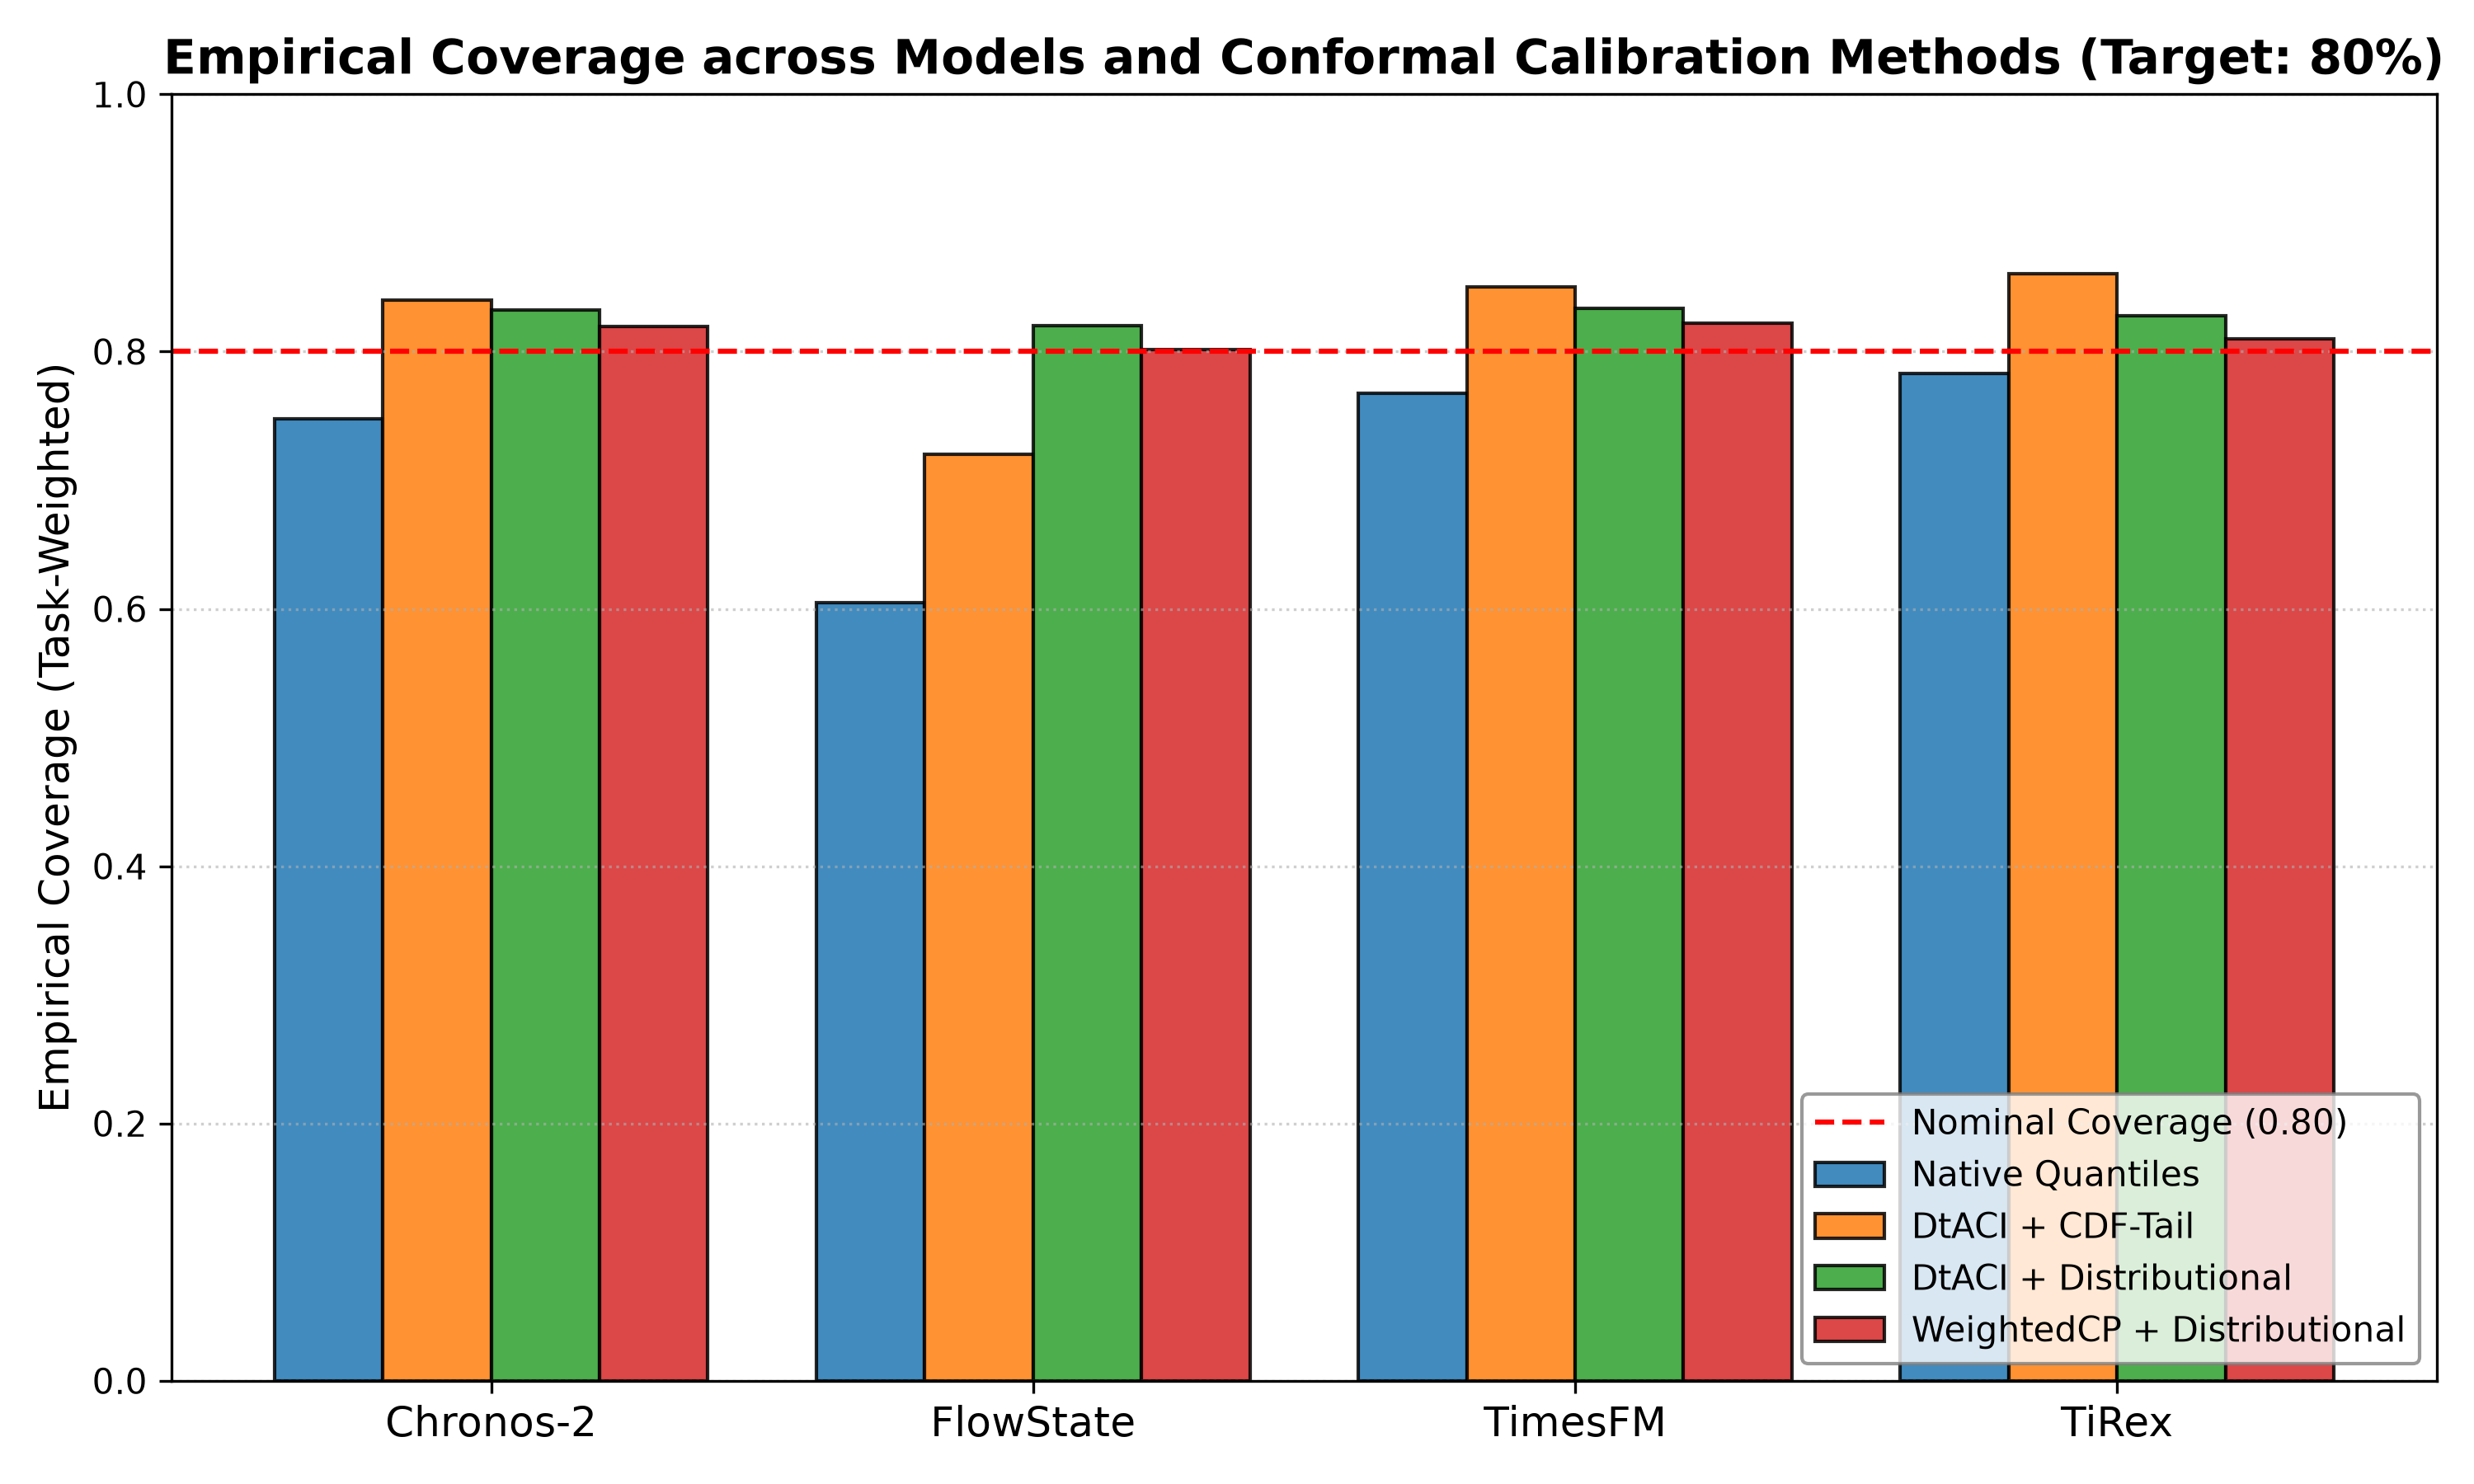
\includegraphics[width=0.9\textwidth]{coverage_comparison.png}
	\caption{Empirical task-weighted coverage of native quantiles and selected conformal calibration configurations across all four evaluation models on FEV-bench mini at \(\alpha=0.20\) (nominal target \(1-\alpha=0.80\)). The red dashed line denotes the target coverage.}
	\label{fig:coverage_comparison}
\end{figure}

\subsection{Coverage of Base FMs vs. CP Calibration}
Our analysis reveals that native, out-of-the-box TSFM quantiles are consistently poorly calibrated and typically underestimate uncertainty in zero-shot environments. For example, FlowState exhibits a severe native coverage gap, reaching only \(60.5\%\) task-weighted coverage against the target \(80\%\). Chronos-2 (\(74.7\%\)) and TimesFM (\(76.6\%\)) also fall short of the nominal target.

Applying conformal prediction (CP) methods significantly improves empirical coverage, closing the calibration gap. Most notably, CP configurations utilizing the \texttt{cdf\_tail} and \texttt{distributional} nonconformity scores consistently provide the best empirical coverage, bringing it much closer to the nominal target without excessive overcoverage. For instance, on FlowState, \textbf{DtACI + Distributional} elevates coverage from \(60.5\%\) to \(82.0\%\) (task-weighted), while \textbf{WeightedCP + Distributional} achieves \(80.2\%\), both keeping scaled interval widths modest (under \(2.0\times\) the native width). For TimesFM, \textbf{SplitCP + CDF-Tail} improves coverage to \(83.1\%\), while \textbf{DtACI + CDF-Tail} achieves \(85.0\%\).

The success of the \texttt{cdf\_tail} and \texttt{distributional} scores stems from their mathematical formulation: rather than relying on point-forecast residuals (like \texttt{abs}) or only two boundary quantiles (like \texttt{cqr}), they utilize the \textit{entire predicted quantile grid} output by the foundation models. By interpolating the cumulative distribution function (CDF) or computing the cumulative pinball loss, they calibrate tail probabilities directly, enabling robust quantile/probability-band inversions that naturally respect distribution limits and adapt dynamically without bloating interval widths.

\subsection{TiRex: Robust Native Quantiles}
A key standout in our study is \textbf{TiRex}. Unlike the transformer and state-space architectures, TiRex's native quantiles are remarkably robust, achieving \(78.3\%\) task-weighted and \(80.2\%\) series-weighted coverage out-of-the-box. This represents near-perfect calibration natively.

Consequently, post-hoc conformal prediction methods do not really improve upon TiRex's native quantiles. In fact, applying adaptive methods like DtACI or ACI to TiRex slightly over-corrects, shifting coverage to \(84\%\)--\(86\%\) while unnecessarily widening the intervals (\(21\%\) to \(26\%\) wider). The intrinsic calibration of TiRex can be attributed to its underlying xLSTM recurrent state-tracking, which excels at retaining local history and context, leading to highly stable and precise in-context quantile estimates that generalize effectively in zero-shot settings without post-hoc correction.

\subsection{Cross-Model Interval Width Comparison}
Tables~\ref{tab:calibration_results_part1} and~\ref{tab:calibration_results_part2} report interval widths scaled relative to each model's own native quantile baseline, which reveals the relative cost of post-hoc calibration within each model but does not allow direct comparison of interval efficiency \textit{across} models. To enable such comparison, we introduce a \textit{task-normalized} width metric: for each task, all interval widths (native and CP-calibrated) are divided by the mean native width across all four models on that task. This shared denominator places all models on a common scale per task, and we aggregate via task-weighted averaging. Results are presented in Table~\ref{tab:cross_model}.

\begin{table}[ht]
	\centering
	\caption{Cross-model comparison of coverage and interval width efficiency on FEV-bench mini (\(\alpha=0.2\)). Widths are task-normalized: for each task, all widths are divided by the mean native width across the four models, enabling direct cross-model comparison. Bold indicates the best model per configuration (closest to \(0.80\) for coverage, narrowest for width). Excludes failure cases.}
	\label{tab:cross_model}
	\setlength{\tabcolsep}{4pt}
	\resizebox{\textwidth}{!}{%
		\begin{tabular}{lcccccccc}
			\hline
			Calibration Method          & \multicolumn{4}{c}{Coverage \(\uparrow\)} & \multicolumn{4}{c}{Normalized Width \(\downarrow\)}                                                                                                    \\
			& Chronos-2                                 & FlowState                                           & TimesFM   & TiRex              & Chronos-2 & FlowState          & TimesFM            & TiRex     \\
			\hline
			Native Quantiles            & \(0.747\)                                 & \(0.605\)                                           & \(0.766\) & \(\mathbf{0.783}\) & \(1.062\) & \(\mathbf{0.773}\) & \(1.036\)          & \(1.129\) \\
			\hline
			SplitCP + CDF-Tail          & \(\mathbf{0.825}\)                        & \(0.709\)                                           & \(0.834\) & \(0.844\)          & \(1.284\) & \(\mathbf{0.983}\) & \(1.276\)          & \(1.336\) \\
			ACI + CDF-Tail              & \(\mathbf{0.834}\)                        & \(0.720\)                                           & \(0.841\) & \(0.850\)          & \(1.331\) & \(\mathbf{1.000}\) & \(1.296\)          & \(1.381\) \\
			DtACI + CDF-Tail            & \(\mathbf{0.844}\)                        & \(0.721\)                                           & \(0.853\) & \(0.864\)          & \(1.368\) & \(\mathbf{1.002}\) & \(1.342\)          & \(1.441\) \\
			WeightedCP + Distributional & \(0.825\)                                 & \(\mathbf{0.807}\)                                  & \(0.826\) & \(0.813\)          & \(1.371\) & \(1.347\)          & \(\mathbf{1.320}\) & \(1.365\) \\
			DtACI + Distributional      & \(0.841\)                                 & \(\mathbf{0.828}\)                                  & \(0.842\) & \(0.836\)          & \(1.546\) & \(1.538\)          & \(\mathbf{1.502}\) & \(1.561\) \\
			\hline
		\end{tabular}%
	}
\end{table}

The cross-model comparison reveals a clear coverage--width tradeoff. FlowState produces the narrowest intervals across all configurations---its native quantiles are only \(0.773\times\) the cross-model mean---but this comes at the cost of the worst native coverage (\(60.5\%\)), indicating its quantile estimates are systematically too tight. Even after CP correction with \texttt{cdf\_tail} scores, FlowState's intervals remain the narrowest (\(0.98\)--\(1.00\times\) the cross-model mean) but its coverage still lags behind the other models (\(70.9\%\)--\(72.1\%\)). Only the more aggressive \texttt{distributional} score family successfully closes FlowState's coverage gap to the \(80\%\) target, but at the expense of roughly doubling its native interval width.

Conversely, TiRex produces the widest native intervals (\(1.129\times\) the cross-model mean) but achieves the best native coverage (\(78.3\%\)). This suggests TiRex's xLSTM architecture trades interval tightness for calibration accuracy---a favorable tradeoff in practice. Chronos-2 and TimesFM occupy the middle ground on both axes. Notably, the relative cost of CP calibration (the width increase factor from native to CP) is remarkably consistent across Chronos-2, TimesFM, and TiRex for \texttt{cdf\_tail} scores (\(\approx 1.2\)--\(1.3\times\) their own native width), while FlowState pays a proportionally larger penalty (\(\approx 1.3\times\) for \texttt{cdf\_tail}, \(\approx 1.7\)--\(1.9\times\) for \texttt{distributional}) because its native intervals are so severely miscalibrated.

\subsection{Pretraining Insights on \texttt{proenfo\_gfc14}} \label{subsec:pretraining_gfc14}
The evaluation suite contains the \texttt{proenfo\_gfc14} task, which originates from the Global Energy Forecasting Competition 2014 (GEFCom 2014) wind, solar, or load forecasting challenges. Crucially, both \textbf{TimesFM} and \textbf{FlowState} were pretrained on this dataset during their respective foundation-level training phases, while Chronos-2 and TiRex have not seen this task. This allows us to observe how foundation-level pretraining affects zero-shot (or rather, in-distribution) probabilistic calibration.

For TimesFM, pretraining translates to exemplary in-distribution calibration natively. At nominal \(80\%\) coverage (\(\alpha=0.2\)), TimesFM's native quantiles achieve an empirical coverage of \textbf{exactly 0.800} (80.0\%) with a highly efficient average interval width of \(169.67\) and a Winkler score of \(231.45\). This is in stark contrast to Chronos-2 and TiRex, which have not been trained on this task and exhibit native undercoverage (\(72.1\%\) and \(75.3\%\), respectively) alongside significantly wider intervals (\(376.33\) and \(446.84\), respectively). This proves that pretraining enables the model's internal representations to perfectly learn the underlying data-generating process, leading to optimal statistical efficiency (tightest intervals that still satisfy the coverage constraint).

Conversely, FlowState presents a highly contrasting insight. Despite being pretrained on \texttt{proenfo\_gfc14}, FlowState's native quantiles suffer from severe undercoverage, reaching only \(0.531\) (53.1\%) empirical coverage due to excessively over-confident and narrow native intervals (average width of \(97.43\)). This demonstrates that pretraining on a dataset does not guarantee valid native quantile calibration if the underlying architecture or training objectives bias the model toward over-confidence. For FlowState, post-hoc conformal calibration is absolutely vital: applying conformal methods like \textbf{ACI + IQR-Scaled} successfully expands the interval width to \(150.96\), boosting empirical coverage to \(0.720\) and reducing the Winkler score from \(374.09\) to \(330.63\).

Furthermore, analyzing this task at \(\alpha = 0.1\) (nominal \(90\%\) coverage) highlights a key technical benefit of conformal prediction. Because TimesFM, TiRex, and FlowState natively only output quantiles up to \(0.9\) and down to \(0.1\), their native prediction interval is structurally limited to \(80\%\) coverage, yielding identical native results at both \(\alpha = 0.1\) and \(\alpha = 0.2\). Conformal prediction successfully overcomes this architectural limitation by scaling these core quantiles dynamically: at \(\alpha=0.1\), \textbf{TrailingWindow + CQR} and \textbf{WeightedCP + Distributional} successfully calibrate TimesFM to \textbf{91.0\%} and \textbf{92.4\%} empirical coverage, respectively, bypassing the base model's static quantile boundaries.

\subsection{Computational Complexity: Inference and Calibration Runtimes} \label{subsec:runtimes}
To provide a complete practical assessment of the evaluated foundation models and conformal prediction methods, we report their cumulative execution times across the \texttt{fev-bench mini} test suite.

First, we measure the raw foundation model inference times (the time required to generate point forecasts and quantile distribution predictions). \textbf{Chronos-2} is the most computationally efficient, requiring only \(262.55\) seconds of cumulative inference time, thanks to its streamlined T5 decoder token-prediction architecture. \textbf{TiRex} and \textbf{FlowState} follow at \(1,521.56\) seconds and \(1,925.09\) seconds, respectively. \textbf{TimesFM} is the slowest model, requiring \(2,831.97\) seconds (nearly \(47\) minutes) of cumulative inference, which is attributed to its multi-layer patching MLP-Transformer design and sequence-by-sequence decoding mechanism.

Second, we analyze the cumulative post-hoc calibration runtimes across all evaluated tasks, models, and scores per conformal prediction method. The static and lightweight methods add negligible overhead: \textbf{TrailingWindow} (\(7,650.01\) s), \textbf{PID} (\(7,692.15\) s), \textbf{ACI} (\(7,782.25\) s), \textbf{SplitCP} (\(8,924.94\) s), and \textbf{AcMCP} (\(9,138.17\) s) each require approximately \(2.1\) to \(2.5\) hours of cumulative runtimes across the entire high-dimensional search space. \textbf{WeightedCP} requires \(16,031.60\) seconds (\(\approx 4.45\) hours) due to the overhead of computing time-decaying weighted empirical quantiles. The most complex adaptive methods exhibit significant computational bottlenecks: \textbf{AgACI} (Aggregated ACI) requires \(30,452.57\) seconds (\(\approx 8.46\) hours) due to window-ensemble updates, while \textbf{DtACI} (Double-tracked ACI) is the slowest by far, requiring \(80,981.99\) seconds (\(\approx 22.49\) hours) due to the sequential dual-feedback tracking and multivariate threshold updates. This highlights that while advanced adaptive methods like DtACI achieve superior coverage on non-stationary streams, they incur substantial computational overhead in large-scale deployment compared to static SplitCP.

\subsection{The Surprising Competitiveness of Static SplitCP}
In time series forecasting—where data is characteristically non-stationary—strictly static conformal prediction methods like SplitCP are generally expected to perform poorly because they do not adapt to distribution shifts or volatility changes over time. However, our empirical results in Table~\ref{tab:calibration_results_part1} and Table~\ref{tab:calibration_results_part2} show that \textbf{SplitCP + CDF-Tail} is remarkably competitive, frequently outperforming complex adaptive online methods (e.g., achieving the best series-weighted coverage of \(80.5\%\) and \(82.6\%\) on Chronos-2 and TimesFM, respectively, while maintaining the narrowest interval widths). We identify three key factors explaining this behavior:
\begin{enumerate}
	\item \textbf{Extremely Short Evaluation Sequences}: Across the FEV-bench mini tasks, the test evaluation set lengths are very short, typically ranging between \(5\) and \(20\) windows (often exactly \(20\)). Over such short periods, significant non-stationary drift has little to no opportunity to manifest, meaning the exchangeability assumption between the calibration and test sets holds exceptionally well.
	\item \textbf{Variance Inflation in Online Updates}: Adaptive online methods (such as ACI or DtACI) update their adjustment threshold sequentially at each step based on local feedback. Over short test horizons, this feedback loop has high variance and can over-react to random local noise or individual outliers. This introduces variance inflation (wider intervals and higher Winkler scores) without improving coverage. In contrast, SplitCP's static threshold acts as a stable estimator.
	\item \textbf{Synergy of Distributional Scores with TSFM Adaptability}: SplitCP is paired with the \texttt{cdf\_tail} score, which leverages the full predicted quantile grid. Because the base TSFMs (e.g., Chronos-2, TimesFM) are highly robust and already capture time-varying patterns, seasonality, and local volatility in-context, the residuals of the distributional nonconformity scores are clean and stationary. A static global correction is therefore sufficient.
\end{enumerate}

\subsection{Task-Weighted vs. Series-Weighted Evaluation}
An essential methodological insight from our study is the stark contrast between task-weighted and series-weighted aggregation.
\begin{itemize}
	\item \textbf{Series-Weighted Evaluation} assigns equal weight to every individual time-series in the meta-dataset. As a result, the aggregated metrics are heavily dominated by a few very large datasets (such as \texttt{rossmann} with \(11,150\) series or \texttt{boomlet} with thousands). Performance on smaller datasets with only a few series is effectively silenced.
	\item \textbf{Task-Weighted Evaluation} calculates the performance metric within each dataset (task) first, and then computes an unweighted average across all tasks. This treats every dataset---representing distinct domains, sampling frequencies, and forecasting horizons---equally.
\end{itemize}
We observe that series-weighted coverage is often higher than task-weighted coverage (e.g., FlowState native coverage jumps from \(60.5\%\) task-weighted to \(68.5\%\) series-weighted). This indicates that the base models perform better on the massive, standard datasets that dominate series-weighted averages, but struggle to generalize to the smaller, more challenging niche datasets. Task-weighted evaluation provides a much more honest and rigorous representation of zero-shot model generalization across diverse, out-of-distribution domains.

\subsection{Failure Cases of Conformal Calibration}
While conformal prediction offers mathematical coverage guarantees, we identify two major failure modes when integrated with pre-trained TSFMs:
\paragraph{Catastrophic Width Explosion}
When adaptive methods like ACI are combined with locally adaptive scaling scores such as \texttt{iqr\_scaled} or \texttt{mad\_scaled}, we observe severe interval inflation, with task-weighted widths exploding to astronomical magnitudes (e.g., \(10^{290}\)!). This catastrophic failure occurs when:
\begin{enumerate}
	\item The denominator scaling factor (the model's native IQR or local MAD) approaches zero in some windows due to degenerate deterministic forecasts, leading to near-division-by-zero.
	\item The feedback loop in ACI continues to aggressively increment the target quantile in response to sequential outliers or non-stationary structural shocks, causing a runaway expansion.
\end{enumerate}
This highlights a major vulnerability in standard online adaptive CP and underscores the necessity of bounding adjustments or utilizing smoother update schemes like DtACI.

\paragraph{Severe Undercoverage with Squared Scores}
Utilizing the \texttt{squared} point residual score (\(s = (y - \hat{y})^2\)) consistently results in catastrophic undercoverage across all models, with task-weighted coverages collapsing to approximately \(35\%\) against the \(80\%\) target. Because squaring nonconformity residuals severely overemphasizes large error outliers, the empirical quantile threshold is skewed outward to accommodate the tail. When inverted, this shrinks the normal-range prediction intervals excessively close to the median for typical, non-outlier test windows, leaving them severely unprotected.

\subsection{Analysis by Task Properties}
Analyzing the calibration dynamics by task characteristics highlights specific regimes of vulnerability:
\paragraph{Number of Calibration Windows}
When the number of calibration windows is extremely limited (e.g., \(N_{\text{cal}} = 2\) or \(90\), where native coverage collapses to \(64.7\%\) and \(56.3\%\), respectively), post-hoc CP becomes absolutely critical. Under these data-constrained regimes, expert-ensemble methods such as \textbf{AgACI} or \textbf{WeightedCP} combined with \texttt{distributional} scores are highly robust, recovering the target \(80\%\) coverage effectively (achieving \(79.9\%\) and \(80.2\%\) coverage, respectively).

\paragraph{Horizon Length}
For very long horizons (e.g., \(H=288\), where native coverage collapses to \(56.3\%\) due to compounding multi-step error accumulation), standard point-prediction CP methods struggle. However, \textbf{WeightedCP + Distributional} successfully models the cumulative uncertainty profile, bringing coverage back to \(80.5\%\). This confirms that CP methods utilizing full-grid predictive distributions are indispensable for managing uncertainty over extended horizons.

\subsection{Theoretical Comparison of Online Calibration Methods under CQR}
\label{subsec:conformal_comparison}

When applying conformalized quantile regression (CQR) scores to pre-trained Time Series Foundation Models (TSFMs) such as Chronos-2, the nonconformity score at time \(t\) for a given horizon step is defined as:
\begin{equation}
	s_t = \max(q_{\text{low}, t} - y_t, \, y_t - q_{\text{high}, t})
\end{equation}
where \(q_{\text{low}, t}\) and \(q_{\text{high}, t}\) represent the native lower and upper quantile predictions. Because the foundation model's native quantile outputs are already pre-calibrated to a target coverage rate of \(1-\alpha\), the distribution of \(s_t\) exhibits a high density (point mass) around \(0\), with a tail of positive values corresponding to rare boundary violations.

Applying adaptive calibration methods to these scores reveals stark differences in performance, particularly when evaluated using the Winkler score:
\begin{equation}
	W_t = (U_t - L_t) + \frac{2}{\alpha} \max(L_t - y_t, \, y_t - U_t, \, 0)
\end{equation}
where \([L_t, U_t]\) is the constructed prediction interval. The major differences between ACI, AgACI, and DtACI are detailed below.

\paragraph{Continuous vs. Binary Feedback}
Adaptive Conformal Inference (ACI) \cite{aci} and its aggregated variant AgACI \cite{agaci} rely on a binary feedback loop:
\begin{equation}
	e_t = \mathbb{I}(s_t > q_t) \in \{0, 1\}
\end{equation}
which updates the nominal parameters via \(\alpha_{t+1} = \alpha_t + \gamma (\alpha - e_t)\). Near the spike at \(0\) in the CQR score distribution, this binary feedback creates severe \textit{on-off oscillations}. Small noise fluctuations induce sequential violations (\(e_t=1\)) followed by consecutive coverages (\(e_t=0\)). This causes the intervals to alternate between being overly wide (inflating the width term of the Winkler score) and overly narrow (incurring the heavy \(\frac{2}{\alpha}\) miscoverage penalty), resulting in a worse Winkler score than the native baseline.

Conversely, DtACI \cite{dtaci} utilizes the continuous empirical error rate \(\beta_t \in [0,1]\) of the new score relative to the rolling window of scores:
\begin{equation}
	\beta_t = \frac{1}{n} \sum_{i=1}^n \mathbb{I}(s_{t-i} > s_t)
\end{equation}
By replacing the binary feedback with a smooth quantile location, DtACI eliminates high-frequency boundary oscillations, leading to stable interval widths.

\paragraph{Parameter Averaging vs. Randomized Sampling}
AgACI aggregates a grid of candidate step-sizes by taking a linear convex combination of the experts' nominal levels:
\begin{equation}
	\alpha_t = \sum_{k=1}^K p_t^k \alpha_t^k
\end{equation}
Because the mapping from the nominal level \(\alpha_t\) to the empirical quantile \(Q(1-\alpha_t)\) is highly non-linear, parameter averaging is mathematically sub-optimal. It often yields biased quantiles that over-cover without optimizing interval efficiency.

DtACI solves this by randomly sampling the expert at each step according to the probability vector \(p_t\). This guarantees that the aggregated sequence inherits the regret bounds of the best performing expert.

\paragraph{Equivalence to Pinball Loss Minimization}
The Winkler score is mathematically equivalent to the pinball loss \(\rho_\alpha(\cdot)\) up to a scaling factor. ACI and AgACI are formulated as reactive controllers that do not optimize a specific loss. DtACI, however, is explicitly framed within the context of online convex optimization, updating its expert weights by minimizing the pinball loss of the empirical error rates:
\begin{equation}
	\ell(\beta_t, \alpha_{\text{exp}}) = \rho_\alpha(\beta_t - \alpha_{\text{exp}})
\end{equation}
Because DtACI directly minimizes the pinball loss of the quantiles, it is theoretically guaranteed to minimize the objective measured by the Winkler score.


\bibliographystyle{alpha}
\bibliography{ref}

\newpage
\appendix
\setcounter{table}{0}
\renewcommand{\thetable}{A\arabic{table}}
\renewcommand{\theHtable}{A\arabic{table}}
\setcounter{figure}{0}
\renewcommand{\thefigure}{A\arabic{figure}}
\renewcommand{\theHfigure}{A\arabic{figure}}

\section{Complete Grid Search Results} \label{sec:appendix_grid_search}
In this appendix, we present the complete empirical results for all \(398\) combinations of base Time Series Foundation Models, conformal prediction methods, and nonconformity score types evaluated on the \texttt{FEV-bench mini} benchmark at a nominal miscoverage level of \(\alpha = 0.2\) (target \(80\%\) coverage).

\subsection{Coverage vs. Width Grid Visualization}
Figure~\ref{fig:appendix_all_results} displays the trade-off between task-weighted empirical coverage and task-weighted scaled interval width across all combinations. In each panel, every marker represents a unique configuration of conformal prediction method and nonconformity score. High-quality configurations cluster near the red dashed nominal coverage target of \(0.80\) while maintaining a small scaled width (closer to \(1.0\)). Configurations that suffer from interval width explosion (scaled width \(> 100\)) are clipped and plotted at the far-right edge of the subplots (indicated by 'x' markers).

\begin{figure}[!ht]
	\centering
	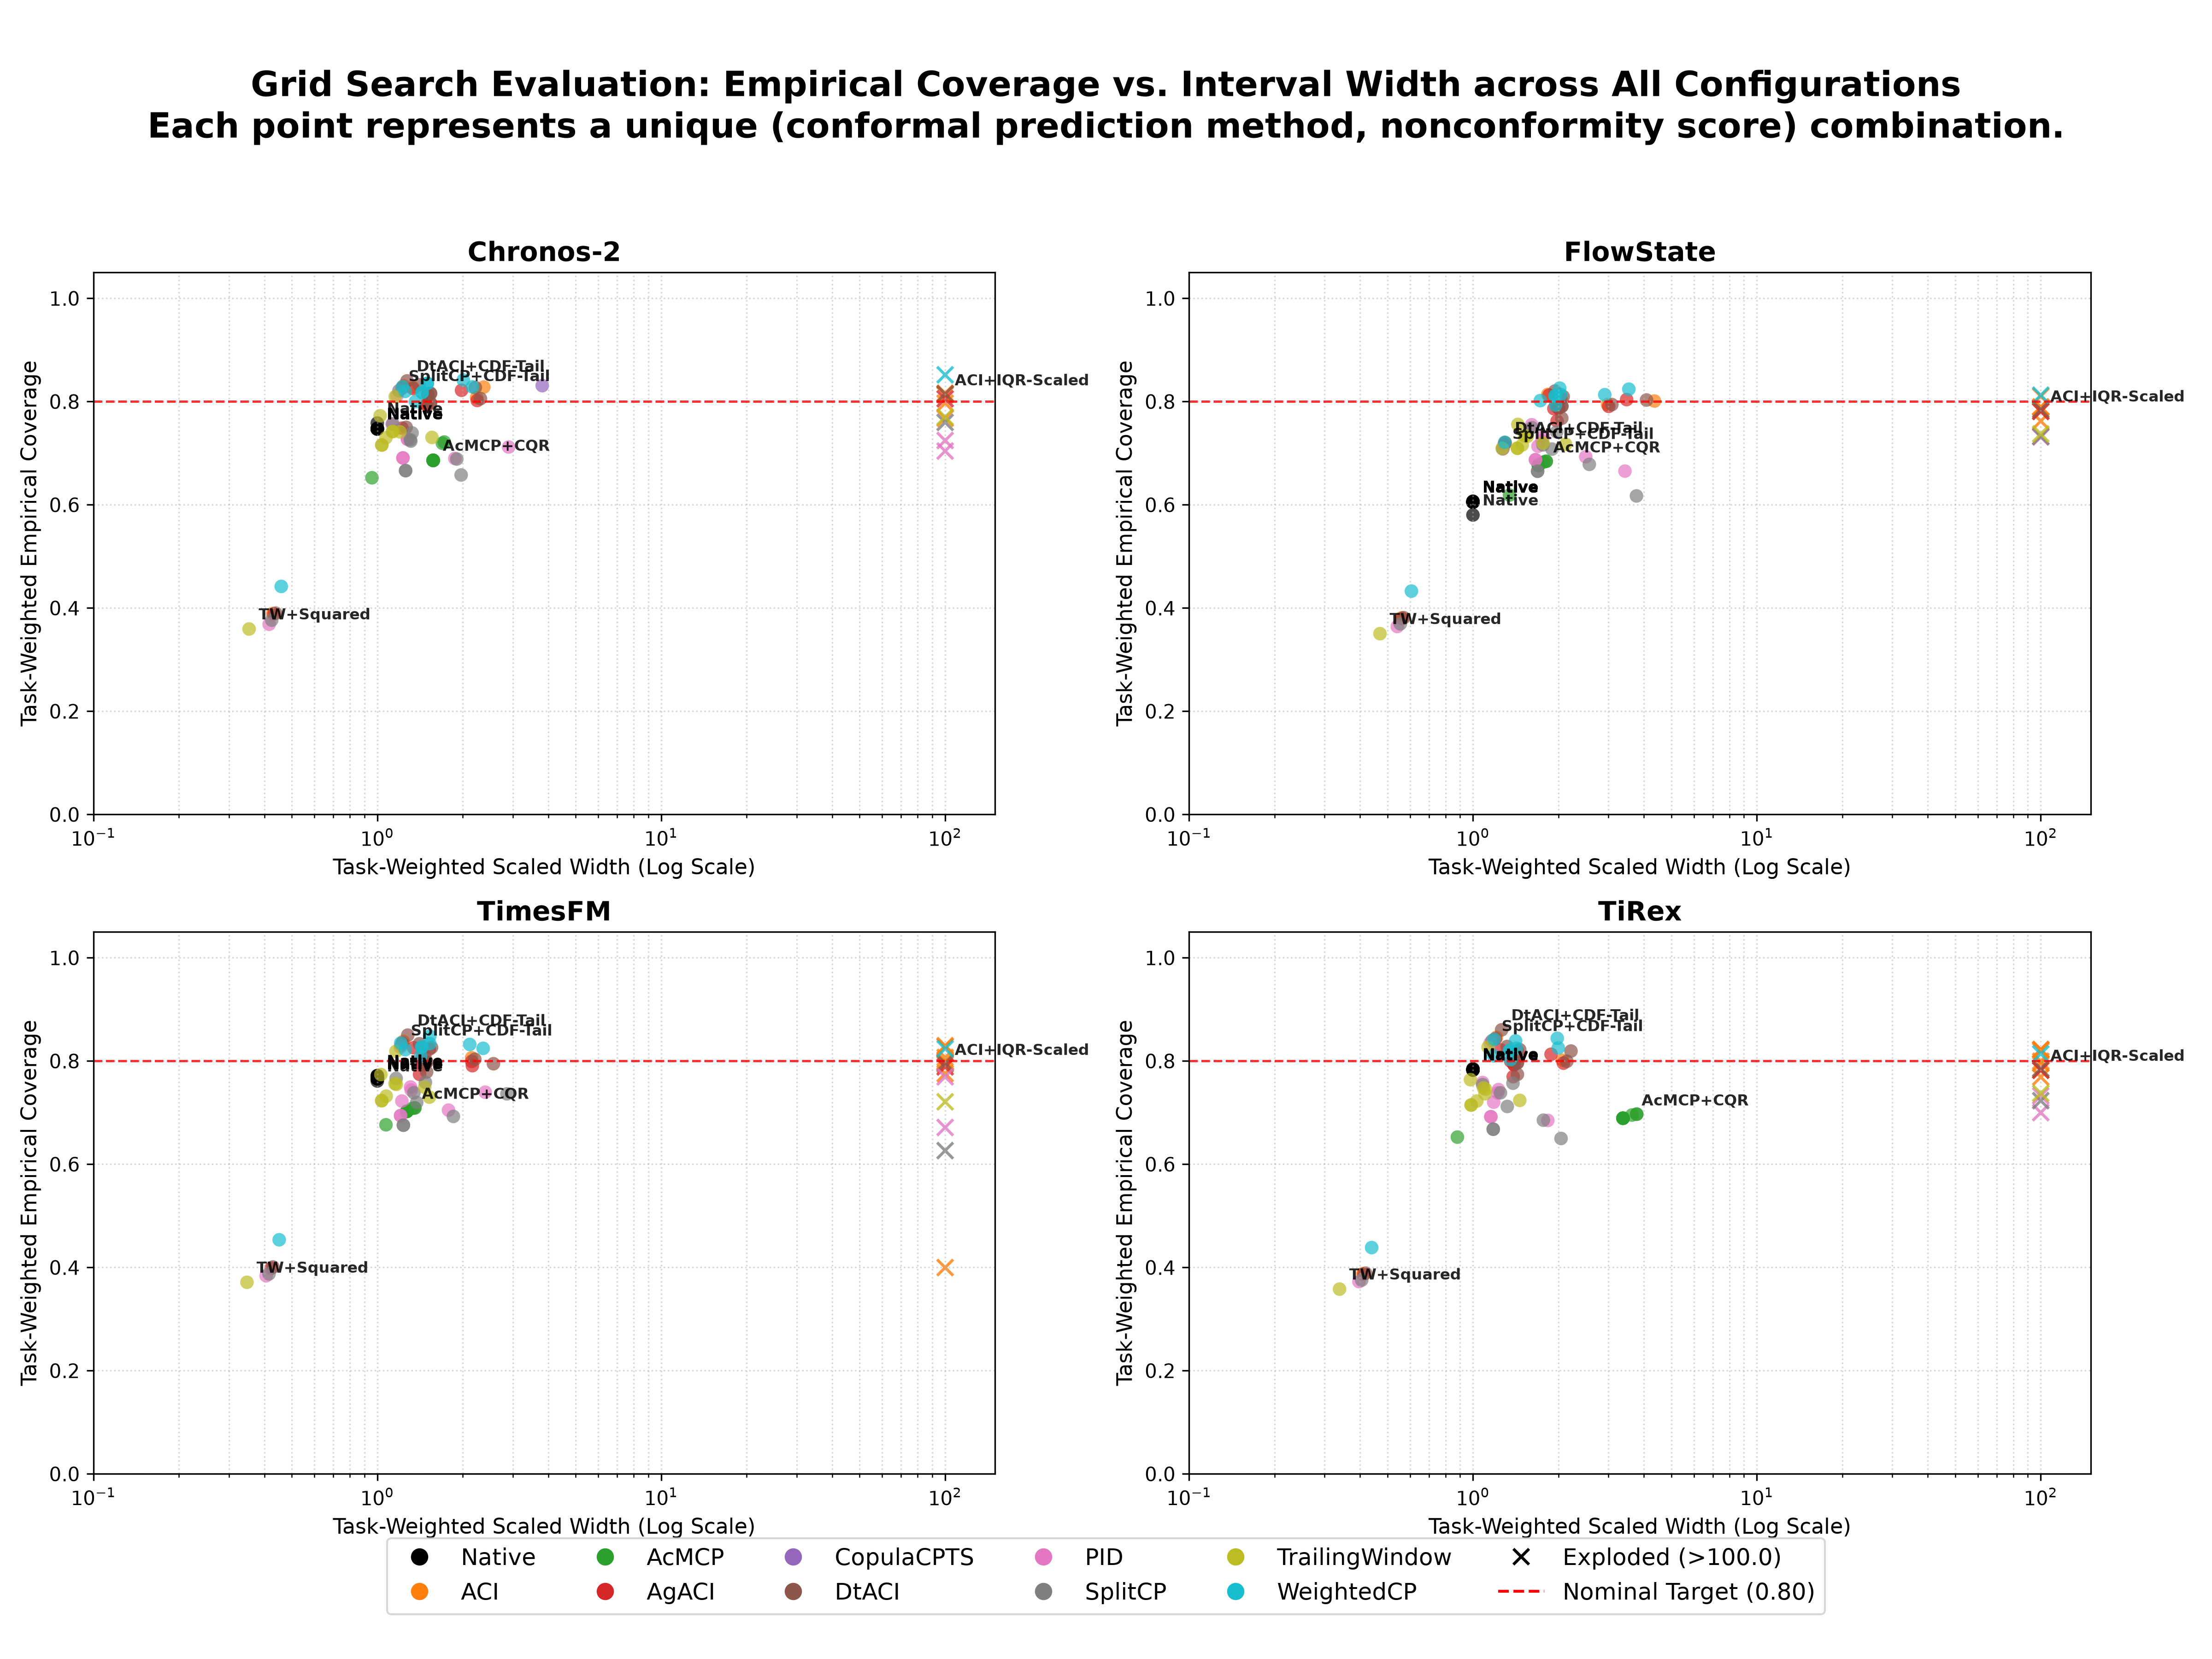
\includegraphics[width=0.9\textwidth]{appendix_all_results.png}
	\caption{Task-weighted empirical coverage vs. task-weighted scaled interval width for all evaluated configurations across Chronos-2, FlowState, TimesFM, and TiRex on FEV-bench mini (\(\alpha=0.2\)). The red dashed line denotes the target coverage of \(80\%\).}
	\label{fig:appendix_all_results}
\end{figure}

\clearpage

% Appendix tables generated automatically by generate_appendix.py
% Contains all model/method/score combinations

\subsection{Complete Results for Chronos-2}
The complete evaluation results of all conformal prediction configurations for \textbf{Chronos-2} on FEV-bench mini at $\alpha=0.2$ are presented in Table~\ref{tab:all_results_chronos2}. Widths are scaled relative to the model's native baseline.

\begin{longtable}{lcccc}
	\caption{All conformal prediction configurations for Chronos-2 on FEV-bench mini ($\alpha=0.2$, Nominal Coverage $1-\alpha=0.80$). columns report Task-Weighted (Task) and Series-Weighted (Series) aggregations.}\\
	\label{tab:all_results_chronos2}\\
	\hline
	Calibration Method & \multicolumn{2}{c}{Coverage $\uparrow$} & \multicolumn{2}{c}{Scaled Width $\downarrow$} \\
 & Task & Series & Task & Series \\
	\hline
	\endfirsthead
	\multicolumn{5}{c}{\tablename\ \thetable\ -- Continued from previous page} \\
	\hline
	Calibration Method & \multicolumn{2}{c}{Coverage $\uparrow$} & \multicolumn{2}{c}{Scaled Width $\downarrow$} \\
 & Task & Series & Task & Series \\
	\hline
	\endhead
	\hline \multicolumn{5}{r}{{Continued on next page}} \\
	\endfoot
	\hline
	\endlastfoot
	ACI + abs & 0.768 & 0.754 & $3.23 \times 10^{285}$ & $3.23 \times 10^{286}$ \\
	ACI + cdf-tail & 0.831 & 0.831 & $1.238$ & $1.251$ \\
	ACI + cqr & 0.816 & 0.733 & $7.47 \times 10^{213}$ & $6.02 \times 10^{214}$ \\
	ACI + diff & 0.808 & 0.748 & $2.238$ & $2.206$ \\
	ACI + distributional & 0.828 & 0.848 & $1.331$ & $1.773$ \\
	ACI + iqr-scaled & 0.813 & 0.761 & $1.08 \times 10^{289}$ & $1.04 \times 10^{290}$ \\
	ACI + log & 0.828 & 0.804 & $2.372$ & $2.890$ \\
	ACI + mad-scaled & 0.797 & 0.733 & $1.495$ & $1.520$ \\
	ACI + scaled-cqr & 0.816 & 0.733 & $8.60 \times 10^{288}$ & $6.93 \times 10^{289}$ \\
	ACI + signed & 0.797 & 0.733 & $7.47 \times 10^{213}$ & $6.02 \times 10^{214}$ \\
	ACI + squared & 0.389 & 0.110 & $0.428$ & $0.139$ \\
	AcMCP + abs & 0.722 & 0.735 & $1.721$ & $1.520$ \\
	AcMCP + cdf-tail & 0.686 & 0.634 & $1.573$ & $1.188$ \\
	AcMCP + cqr & 0.686 & 0.634 & $1.573$ & $1.188$ \\
	AcMCP + diff & 0.686 & 0.634 & $1.573$ & $1.188$ \\
	AcMCP + distributional & 0.686 & 0.634 & $1.573$ & $1.188$ \\
	AcMCP + iqr-scaled & 0.719 & 0.696 & $1.696$ & $1.389$ \\
	AcMCP + log & 0.652 & 0.547 & $0.957$ & $0.782$ \\
	AcMCP + mad-scaled & 0.686 & 0.634 & $1.573$ & $1.188$ \\
	AcMCP + scaled-cqr & 0.686 & 0.634 & $1.573$ & $1.188$ \\
	AcMCP + signed & 0.686 & 0.634 & $1.573$ & $1.188$ \\
	AcMCP + squared & 0.686 & 0.634 & $1.573$ & $1.188$ \\
	AgACI + abs & 0.748 & 0.749 & $1.222$ & $1.377$ \\
	AgACI + cdf-tail & 0.826 & 0.830 & $1.225$ & $1.244$ \\
	AgACI + cqr & 0.813 & 0.731 & $1.508$ & $1.478$ \\
	AgACI + diff & 0.802 & 0.745 & $2.248$ & $2.194$ \\
	AgACI + distributional & 0.825 & 0.847 & $1.335$ & $1.793$ \\
	AgACI + iqr-scaled & 0.805 & 0.758 & $1.25 \times 10^{7}$ & $1.20 \times 10^{8}$ \\
	AgACI + log & 0.822 & 0.798 & $1.980$ & $2.432$ \\
	AgACI + mad-scaled & 0.794 & 0.731 & $1.494$ & $1.504$ \\
	AgACI + scaled-cqr & 0.813 & 0.731 & $1.508$ & $1.478$ \\
	AgACI + signed & 0.794 & 0.731 & $1.494$ & $1.504$ \\
	AgACI + squared & 0.389 & 0.110 & $0.432$ & $0.140$ \\
	CopulaCPTS + joint & 0.831 & 0.915 & $3.810$ & $3.888$ \\
	DtACI + abs & 0.750 & 0.757 & $1.264$ & $1.423$ \\
	DtACI + cdf-tail & 0.840 & 0.834 & $1.273$ & $1.264$ \\
	DtACI + cqr & 0.815 & 0.731 & $1.540$ & $1.477$ \\
	DtACI + diff & 0.806 & 0.745 & $2.308$ & $2.195$ \\
	DtACI + distributional & 0.833 & 0.849 & $1.402$ & $1.836$ \\
	DtACI + iqr-scaled & 0.815 & 0.770 & $1.23 \times 10^{7}$ & $1.15 \times 10^{8}$ \\
	DtACI + log & 0.827 & 0.800 & $2.213$ & $2.662$ \\
	DtACI + mad-scaled & 0.797 & 0.731 & $1.538$ & $1.504$ \\
	DtACI + scaled-cqr & 0.816 & 0.731 & $1.539$ & $1.478$ \\
	DtACI + signed & 0.796 & 0.731 & $1.539$ & $1.506$ \\
	DtACI + squared & 0.390 & 0.109 & $0.439$ & $0.142$ \\
	Native Quantiles & 0.747 & 0.729 & $1.000$ & $1.000$ \\
	PID + abs & 0.712 & 0.687 & $2.901$ & $2.817$ \\
	PID + cdf-tail & 0.811 & 0.805 & $1.172$ & $1.167$ \\
	PID + cqr & 0.727 & 0.532 & $1.277$ & $0.934$ \\
	PID + diff & 0.704 & 0.514 & $2.92 \times 10^{285}$ & $2.35 \times 10^{286}$ \\
	PID + distributional & 0.756 & 0.754 & $1.128$ & $1.457$ \\
	PID + iqr-scaled & 0.725 & 0.604 & $1.29 \times 10^{7}$ & $1.24 \times 10^{8}$ \\
	PID + log & 0.690 & 0.605 & $1.875$ & $1.976$ \\
	PID + mad-scaled & 0.691 & 0.511 & $1.231$ & $0.976$ \\
	PID + scaled-cqr & 0.727 & 0.532 & $1.278$ & $0.936$ \\
	PID + signed & 0.691 & 0.511 & $1.231$ & $0.976$ \\
	PID + squared & 0.369 & 0.103 & $0.416$ & $0.134$ \\
	SplitCP + abs & 0.739 & 0.682 & $1.325$ & $1.368$ \\
	SplitCP + cdf-tail & 0.821 & 0.805 & $1.192$ & $1.170$ \\
	SplitCP + cqr & 0.726 & 0.480 & $1.307$ & $0.869$ \\
	SplitCP + diff & 0.689 & 0.456 & $1.905$ & $1.419$ \\
	SplitCP + distributional & 0.757 & 0.736 & $1.134$ & $1.484$ \\
	SplitCP + iqr-scaled & 0.760 & 0.555 & $1.17 \times 10^{7}$ & $1.12 \times 10^{8}$ \\
	SplitCP + log & 0.658 & 0.529 & $1.974$ & $2.085$ \\
	SplitCP + mad-scaled & 0.666 & 0.440 & $1.258$ & $0.927$ \\
	SplitCP + scaled-cqr & 0.723 & 0.478 & $1.312$ & $0.868$ \\
	SplitCP + signed & 0.666 & 0.440 & $1.258$ & $0.927$ \\
	SplitCP + squared & 0.377 & 0.104 & $0.425$ & $0.138$ \\
	TrailingWindow + abs & 0.730 & 0.746 & $1.073$ & $1.230$ \\
	TrailingWindow + cdf-tail & 0.809 & 0.805 & $1.156$ & $1.149$ \\
	TrailingWindow + cqr & 0.742 & 0.683 & $1.132$ & $1.137$ \\
	TrailingWindow + diff & 0.731 & 0.703 & $1.558$ & $1.735$ \\
	TrailingWindow + distributional & 0.772 & 0.773 & $1.023$ & $1.159$ \\
	TrailingWindow + iqr-scaled & 0.770 & 0.727 & $8.20 \times 10^{6}$ & $7.86 \times 10^{7}$ \\
	TrailingWindow + log & 0.741 & 0.720 & $1.201$ & $1.249$ \\
	TrailingWindow + mad-scaled & 0.716 & 0.688 & $1.037$ & $1.150$ \\
	TrailingWindow + scaled-cqr & 0.742 & 0.683 & $1.131$ & $1.136$ \\
	TrailingWindow + signed & 0.716 & 0.688 & $1.038$ & $1.150$ \\
	TrailingWindow + squared & 0.359 & 0.101 & $0.353$ & $0.114$ \\
	WeightedCP + abs & 0.800 & 0.839 & $1.363$ & $1.890$ \\
	WeightedCP + cdf-tail & 0.829 & 0.840 & $1.226$ & $1.269$ \\
	WeightedCP + cqr & 0.835 & 0.857 & $1.500$ & $2.038$ \\
	WeightedCP + diff & 0.828 & 0.850 & $2.164$ & $2.945$ \\
	WeightedCP + distributional & 0.820 & 0.881 & $1.254$ & $1.650$ \\
	WeightedCP + iqr-scaled & 0.852 & 0.874 & $1.31 \times 10^{7}$ & $1.54 \times 10^{8}$ \\
	WeightedCP + log & 0.842 & 0.880 & $2.009$ & $2.721$ \\
	WeightedCP + mad-scaled & 0.818 & 0.845 & $1.438$ & $2.033$ \\
	WeightedCP + scaled-cqr & 0.835 & 0.857 & $1.500$ & $2.038$ \\
	WeightedCP + signed & 0.818 & 0.845 & $1.438$ & $2.033$ \\
	WeightedCP + squared & 0.442 & 0.182 & $0.459$ & $0.212$ \\
\end{longtable}

\subsection{Complete Results for FlowState}
The complete evaluation results of all conformal prediction configurations for \textbf{FlowState} on FEV-bench mini at $\alpha=0.2$ are presented in Table~\ref{tab:all_results_flowstate}. Widths are scaled relative to the model's native baseline.

\begin{longtable}{lcccc}
	\caption{All conformal prediction configurations for FlowState on FEV-bench mini ($\alpha=0.2$, Nominal Coverage $1-\alpha=0.80$). columns report Task-Weighted (Task) and Series-Weighted (Series) aggregations.}\\
	\label{tab:all_results_flowstate}\\
	\hline
	Calibration Method & \multicolumn{2}{c}{Coverage $\uparrow$} & \multicolumn{2}{c}{Scaled Width $\downarrow$} \\
 & Task & Series & Task & Series \\
	\hline
	\endfirsthead
	\multicolumn{5}{c}{\tablename\ \thetable\ -- Continued from previous page} \\
	\hline
	Calibration Method & \multicolumn{2}{c}{Coverage $\uparrow$} & \multicolumn{2}{c}{Scaled Width $\downarrow$} \\
 & Task & Series & Task & Series \\
	\hline
	\endhead
	\hline \multicolumn{5}{r}{{Continued on next page}} \\
	\endfoot
	\hline
	\endlastfoot
	ACI + abs & 0.762 & 0.724 & $4.63 \times 10^{276}$ & $3.94 \times 10^{277}$ \\
	ACI + cdf-tail & 0.720 & 0.792 & $1.296$ & $1.261$ \\
	ACI + cqr & 0.788 & 0.733 & $1.08 \times 10^{286}$ & $9.49 \times 10^{286}$ \\
	ACI + diff & 0.794 & 0.736 & $2.981$ & $2.526$ \\
	ACI + distributional & 0.814 & 0.835 & $1.836$ & $1.992$ \\
	ACI + iqr-scaled & 0.781 & 0.736 & $4.93 \times 10^{290}$ & $4.60 \times 10^{291}$ \\
	ACI + log & 0.801 & 0.799 & $4.359$ & $4.820$ \\
	ACI + mad-scaled & 0.790 & 0.723 & $1.45 \times 10^{217}$ & $1.17 \times 10^{218}$ \\
	ACI + scaled-cqr & 0.810 & 0.735 & $7.65 \times 10^{289}$ & $6.17 \times 10^{290}$ \\
	ACI + signed & 0.790 & 0.723 & $1.998$ & $1.714$ \\
	ACI + squared & 0.381 & 0.104 & $0.560$ & $0.170$ \\
	AcMCP + abs & 0.684 & 0.636 & $1.812$ & $1.430$ \\
	AcMCP + cdf-tail & 0.676 & 0.582 & $1.702$ & $1.239$ \\
	AcMCP + cqr & 0.683 & 0.615 & $1.774$ & $1.353$ \\
	AcMCP + diff & 0.676 & 0.582 & $1.702$ & $1.239$ \\
	AcMCP + distributional & 0.676 & 0.582 & $1.702$ & $1.239$ \\
	AcMCP + iqr-scaled & 0.684 & 0.636 & $1.812$ & $1.430$ \\
	AcMCP + log & 0.619 & 0.558 & $1.345$ & $1.186$ \\
	AcMCP + mad-scaled & 0.676 & 0.582 & $1.702$ & $1.239$ \\
	AcMCP + scaled-cqr & 0.676 & 0.582 & $1.702$ & $1.239$ \\
	AcMCP + signed & 0.676 & 0.582 & $1.702$ & $1.239$ \\
	AcMCP + squared & 0.676 & 0.582 & $1.702$ & $1.239$ \\
	AgACI + abs & 0.762 & 0.723 & $1.978$ & $1.135$ \\
	AgACI + cdf-tail & 0.717 & 0.790 & $1.289$ & $1.257$ \\
	AgACI + cqr & 0.786 & 0.732 & $1.928$ & $1.675$ \\
	AgACI + diff & 0.791 & 0.734 & $3.007$ & $2.512$ \\
	AgACI + distributional & 0.812 & 0.834 & $1.854$ & $2.016$ \\
	AgACI + iqr-scaled & 0.781 & 0.735 & $24033.8$ & $230257.1$ \\
	AgACI + log & 0.804 & 0.797 & $3.478$ & $3.894$ \\
	AgACI + mad-scaled & 0.787 & 0.721 & $2.003$ & $1.702$ \\
	AgACI + scaled-cqr & 0.806 & 0.734 & $2.040$ & $1.701$ \\
	AgACI + signed & 0.787 & 0.721 & $2.003$ & $1.702$ \\
	AgACI + squared & 0.380 & 0.104 & $0.563$ & $0.170$ \\
	DtACI + abs & 0.768 & 0.733 & $2.055$ & $1.125$ \\
	DtACI + cdf-tail & 0.720 & 0.792 & $1.298$ & $1.262$ \\
	DtACI + cqr & 0.791 & 0.738 & $1.973$ & $1.757$ \\
	DtACI + diff & 0.794 & 0.733 & $3.085$ & $2.516$ \\
	DtACI + distributional & 0.820 & 0.835 & $1.945$ & $2.059$ \\
	DtACI + iqr-scaled & 0.785 & 0.745 & $23566.9$ & $216372.4$ \\
	DtACI + log & 0.803 & 0.795 & $4.087$ & $4.478$ \\
	DtACI + mad-scaled & 0.791 & 0.720 & $2.057$ & $1.703$ \\
	DtACI + scaled-cqr & 0.810 & 0.733 & $2.079$ & $1.699$ \\
	DtACI + signed & 0.791 & 0.720 & $2.055$ & $1.701$ \\
	DtACI + squared & 0.381 & 0.104 & $0.570$ & $0.172$ \\
	Native Quantiles & 0.607 & 0.676 & $1.000$ & $1.000$ \\
	PID + abs & 0.714 & 0.623 & $1.694$ & $0.842$ \\
	PID + cdf-tail & 0.708 & 0.770 & $1.274$ & $1.202$ \\
	PID + cqr & 0.732 & 0.585 & $1.770$ & $0.943$ \\
	PID + diff & 0.693 & 0.503 & $2.496$ & $1.668$ \\
	PID + distributional & 0.755 & 0.725 & $1.610$ & $1.633$ \\
	PID + iqr-scaled & 0.731 & 0.633 & $12827.7$ & $109220.2$ \\
	PID + log & 0.665 & 0.596 & $3.432$ & $3.508$ \\
	PID + mad-scaled & 0.687 & 0.505 & $1.661$ & $1.104$ \\
	PID + scaled-cqr & 0.724 & 0.517 & $1.750$ & $1.099$ \\
	PID + signed & 0.687 & 0.505 & $1.661$ & $1.104$ \\
	PID + squared & 0.364 & 0.098 & $0.541$ & $0.164$ \\
	SplitCP + abs & 0.708 & 0.546 & $1.898$ & $1.372$ \\
	SplitCP + cdf-tail & 0.709 & 0.771 & $1.274$ & $1.205$ \\
	SplitCP + cqr & 0.741 & 0.533 & $1.972$ & $1.234$ \\
	SplitCP + diff & 0.678 & 0.446 & $2.570$ & $1.606$ \\
	SplitCP + distributional & 0.749 & 0.694 & $1.613$ & $1.651$ \\
	SplitCP + iqr-scaled & 0.732 & 0.558 & $18735.6$ & $174497.5$ \\
	SplitCP + log & 0.617 & 0.535 & $3.767$ & $3.787$ \\
	SplitCP + mad-scaled & 0.665 & 0.431 & $1.690$ & $1.051$ \\
	SplitCP + scaled-cqr & 0.716 & 0.469 & $1.765$ & $1.035$ \\
	SplitCP + signed & 0.665 & 0.431 & $1.690$ & $1.051$ \\
	SplitCP + squared & 0.369 & 0.099 & $0.555$ & $0.170$ \\
	TrailingWindow + abs & 0.716 & 0.693 & $1.492$ & $0.963$ \\
	TrailingWindow + cdf-tail & 0.709 & 0.772 & $1.268$ & $1.206$ \\
	TrailingWindow + cqr & 0.732 & 0.697 & $1.552$ & $1.371$ \\
	TrailingWindow + diff & 0.717 & 0.689 & $2.120$ & $1.987$ \\
	TrailingWindow + distributional & 0.756 & 0.758 & $1.439$ & $1.329$ \\
	TrailingWindow + iqr-scaled & 0.737 & 0.707 & $18082.1$ & $166020.6$ \\
	TrailingWindow + log & 0.720 & 0.717 & $1.766$ & $1.862$ \\
	TrailingWindow + mad-scaled & 0.709 & 0.676 & $1.435$ & $1.302$ \\
	TrailingWindow + scaled-cqr & 0.734 & 0.690 & $1.521$ & $1.327$ \\
	TrailingWindow + signed & 0.710 & 0.676 & $1.434$ & $1.302$ \\
	TrailingWindow + squared & 0.350 & 0.096 & $0.470$ & $0.142$ \\
	WeightedCP + abs & 0.793 & 0.821 & $1.953$ & $1.449$ \\
	WeightedCP + cdf-tail & 0.721 & 0.806 & $1.294$ & $1.278$ \\
	WeightedCP + cqr & 0.814 & 0.841 & $2.039$ & $2.382$ \\
	WeightedCP + diff & 0.813 & 0.843 & $2.912$ & $3.509$ \\
	WeightedCP + distributional & 0.802 & 0.861 & $1.727$ & $1.842$ \\
	WeightedCP + iqr-scaled & 0.812 & 0.834 & $20701.3$ & $235637.7$ \\
	WeightedCP + log & 0.824 & 0.882 & $3.541$ & $4.400$ \\
	WeightedCP + mad-scaled & 0.811 & 0.843 & $1.947$ & $2.394$ \\
	WeightedCP + scaled-cqr & 0.826 & 0.861 & $2.021$ & $2.416$ \\
	WeightedCP + signed & 0.811 & 0.843 & $1.947$ & $2.394$ \\
	WeightedCP + squared & 0.433 & 0.173 & $0.607$ & $0.264$ \\
\end{longtable}

\subsection{Complete Results for TimesFM}
The complete evaluation results of all conformal prediction configurations for \textbf{TimesFM} on FEV-bench mini at $\alpha=0.2$ are presented in Table~\ref{tab:all_results_timesfm}. Widths are scaled relative to the model's native baseline.

\begin{longtable}{lcccc}
	\caption{All conformal prediction configurations for TimesFM on FEV-bench mini ($\alpha=0.2$, Nominal Coverage $1-\alpha=0.80$). columns report Task-Weighted (Task) and Series-Weighted (Series) aggregations.}\\
	\label{tab:all_results_timesfm}\\
	\hline
	Calibration Method & \multicolumn{2}{c}{Coverage $\uparrow$} & \multicolumn{2}{c}{Scaled Width $\downarrow$} \\
 & Task & Series & Task & Series \\
	\hline
	\endfirsthead
	\multicolumn{5}{c}{\tablename\ \thetable\ -- Continued from previous page} \\
	\hline
	Calibration Method & \multicolumn{2}{c}{Coverage $\uparrow$} & \multicolumn{2}{c}{Scaled Width $\downarrow$} \\
 & Task & Series & Task & Series \\
	\hline
	\endhead
	\hline \multicolumn{5}{r}{{Continued on next page}} \\
	\endfoot
	\hline
	\endlastfoot
	ACI + abs & 0.775 & 0.726 & $7.82 \times 10^{286}$ & $6.66 \times 10^{287}$ \\
	ACI + cdf-tail & 0.838 & 0.844 & $1.235$ & $1.251$ \\
	ACI + cqr & 0.807 & 0.738 & $5.84 \times 10^{286}$ & $5.15 \times 10^{287}$ \\
	ACI + diff & 0.806 & 0.740 & $2.149$ & $2.211$ \\
	ACI + distributional & 0.830 & 0.835 & $7.11 \times 10^{285}$ & $5.73 \times 10^{286}$ \\
	ACI + iqr-scaled & 0.793 & 0.726 & $1.84 \times 10^{290}$ & $1.72 \times 10^{291}$ \\
	ACI + log & 0.797 & 0.722 & $7.38 \times 10^{7}$ & $4.55 \times 10^{8}$ \\
	ACI + mad-scaled & 0.798 & 0.722 & $8.65 \times 10^{289}$ & $6.97 \times 10^{290}$ \\
	ACI + scaled-cqr & 0.828 & 0.739 & $9.54 \times 10^{288}$ & $7.68 \times 10^{289}$ \\
	ACI + signed & 0.799 & 0.722 & $8.04 \times 10^{286}$ & $6.48 \times 10^{287}$ \\
	ACI + squared & 0.400 & 0.146 & $4.74 \times 10^{138}$ & $3.82 \times 10^{139}$ \\
	AcMCP + abs & 0.709 & 0.671 & $1.356$ & $1.321$ \\
	AcMCP + cdf-tail & 0.702 & 0.618 & $1.271$ & $1.139$ \\
	AcMCP + cqr & 0.708 & 0.650 & $1.327$ & $1.248$ \\
	AcMCP + diff & 0.702 & 0.618 & $1.271$ & $1.139$ \\
	AcMCP + distributional & 0.702 & 0.618 & $1.271$ & $1.139$ \\
	AcMCP + iqr-scaled & 0.709 & 0.671 & $1.356$ & $1.321$ \\
	AcMCP + log & 0.676 & 0.602 & $1.073$ & $1.101$ \\
	AcMCP + mad-scaled & 0.702 & 0.618 & $1.271$ & $1.139$ \\
	AcMCP + scaled-cqr & 0.702 & 0.618 & $1.271$ & $1.139$ \\
	AcMCP + signed & 0.702 & 0.618 & $1.271$ & $1.139$ \\
	AcMCP + squared & 0.702 & 0.618 & $1.271$ & $1.139$ \\
	AgACI + abs & 0.774 & 0.725 & $1.409$ & $1.001$ \\
	AgACI + cdf-tail & 0.835 & 0.842 & $1.224$ & $1.245$ \\
	AgACI + cqr & 0.805 & 0.738 & $1.433$ & $1.493$ \\
	AgACI + diff & 0.799 & 0.738 & $2.152$ & $2.199$ \\
	AgACI + distributional & 0.826 & 0.834 & $1.342$ & $1.799$ \\
	AgACI + iqr-scaled & 0.791 & 0.726 & $2.162$ & $1.973$ \\
	AgACI + log & 0.789 & 0.721 & $7.06 \times 10^{7}$ & $4.34 \times 10^{8}$ \\
	AgACI + mad-scaled & 0.793 & 0.720 & $1.447$ & $1.506$ \\
	AgACI + scaled-cqr & 0.823 & 0.738 & $1.525$ & $1.509$ \\
	AgACI + signed & 0.793 & 0.720 & $1.447$ & $1.506$ \\
	AgACI + squared & 0.399 & 0.146 & $0.423$ & $0.138$ \\
	DtACI + abs & 0.779 & 0.734 & $1.492$ & $0.995$ \\
	DtACI + cdf-tail & 0.850 & 0.848 & $1.280$ & $1.267$ \\
	DtACI + cqr & 0.809 & 0.743 & $1.470$ & $1.583$ \\
	DtACI + diff & 0.803 & 0.738 & $2.205$ & $2.199$ \\
	DtACI + distributional & 0.833 & 0.835 & $1.407$ & $1.845$ \\
	DtACI + iqr-scaled & 0.795 & 0.735 & $2.565$ & $2.125$ \\
	DtACI + log & 0.796 & 0.720 & $7.06 \times 10^{7}$ & $4.34 \times 10^{8}$ \\
	DtACI + mad-scaled & 0.798 & 0.719 & $1.493$ & $1.506$ \\
	DtACI + scaled-cqr & 0.826 & 0.738 & $1.552$ & $1.512$ \\
	DtACI + signed & 0.798 & 0.719 & $1.493$ & $1.506$ \\
	DtACI + squared & 0.401 & 0.146 & $0.429$ & $0.140$ \\
	Native Quantiles & 0.772 & 0.751 & $1.000$ & $1.000$ \\
	PID + abs & 0.722 & 0.632 & $1.221$ & $0.734$ \\
	PID + cdf-tail & 0.827 & 0.825 & $1.205$ & $1.182$ \\
	PID + cqr & 0.750 & 0.607 & $1.309$ & $0.843$ \\
	PID + diff & 0.705 & 0.512 & $1.782$ & $1.492$ \\
	PID + distributional & 0.769 & 0.730 & $8.24 \times 10^{16}$ & $6.64 \times 10^{17}$ \\
	PID + iqr-scaled & 0.740 & 0.631 & $2.399$ & $0.828$ \\
	PID + log & 0.671 & 0.494 & $2.18 \times 10^{6}$ & $1.19 \times 10^{7}$ \\
	PID + mad-scaled & 0.694 & 0.519 & $1.208$ & $0.987$ \\
	PID + scaled-cqr & 0.744 & 0.545 & $1.316$ & $0.997$ \\
	PID + signed & 0.694 & 0.519 & $1.208$ & $0.987$ \\
	PID + squared & 0.384 & 0.141 & $0.406$ & $0.132$ \\
	SplitCP + abs & 0.720 & 0.566 & $1.376$ & $1.243$ \\
	SplitCP + cdf-tail & 0.831 & 0.826 & $1.214$ & $1.188$ \\
	SplitCP + cqr & 0.759 & 0.568 & $1.477$ & $1.116$ \\
	SplitCP + diff & 0.693 & 0.455 & $1.854$ & $1.451$ \\
	SplitCP + distributional & 0.766 & 0.700 & $1.165$ & $1.464$ \\
	SplitCP + iqr-scaled & 0.736 & 0.546 & $2.861$ & $3.840$ \\
	SplitCP + log & 0.626 & 0.430 & $2.25 \times 10^{6}$ & $1.09 \times 10^{7}$ \\
	SplitCP + mad-scaled & 0.676 & 0.447 & $1.235$ & $0.952$ \\
	SplitCP + scaled-cqr & 0.738 & 0.508 & $1.345$ & $0.955$ \\
	SplitCP + signed & 0.676 & 0.447 & $1.235$ & $0.952$ \\
	SplitCP + squared & 0.388 & 0.142 & $0.415$ & $0.136$ \\
	TrailingWindow + abs & 0.732 & 0.696 & $1.075$ & $0.831$ \\
	TrailingWindow + cdf-tail & 0.819 & 0.816 & $1.163$ & $1.147$ \\
	TrailingWindow + cqr & 0.755 & 0.703 & $1.167$ & $1.230$ \\
	TrailingWindow + diff & 0.730 & 0.698 & $1.526$ & $1.740$ \\
	TrailingWindow + distributional & 0.774 & 0.759 & $1.029$ & $1.163$ \\
	TrailingWindow + iqr-scaled & 0.749 & 0.693 & $1.468$ & $1.606$ \\
	TrailingWindow + log & 0.721 & 0.681 & $6.88 \times 10^{7}$ & $4.26 \times 10^{8}$ \\
	TrailingWindow + mad-scaled & 0.723 & 0.677 & $1.036$ & $1.148$ \\
	TrailingWindow + scaled-cqr & 0.756 & 0.695 & $1.154$ & $1.185$ \\
	TrailingWindow + signed & 0.723 & 0.677 & $1.036$ & $1.147$ \\
	TrailingWindow + squared & 0.371 & 0.140 & $0.347$ & $0.113$ \\
	WeightedCP + abs & 0.810 & 0.830 & $1.421$ & $1.236$ \\
	WeightedCP + cdf-tail & 0.835 & 0.854 & $1.209$ & $1.258$ \\
	WeightedCP + cqr & 0.834 & 0.853 & $1.530$ & $2.099$ \\
	WeightedCP + diff & 0.832 & 0.857 & $2.116$ & $3.043$ \\
	WeightedCP + distributional & 0.822 & 0.875 & $1.255$ & $1.647$ \\
	WeightedCP + iqr-scaled & 0.825 & 0.834 & $2.359$ & $5.608$ \\
	WeightedCP + log & 0.824 & 0.892 & $2.65 \times 10^{6}$ & $2.36 \times 10^{7}$ \\
	WeightedCP + mad-scaled & 0.827 & 0.856 & $1.434$ & $2.084$ \\
	WeightedCP + scaled-cqr & 0.848 & 0.876 & $1.531$ & $2.103$ \\
	WeightedCP + signed & 0.827 & 0.856 & $1.434$ & $2.084$ \\
	WeightedCP + squared & 0.454 & 0.242 & $0.451$ & $0.210$ \\
\end{longtable}

\subsection{Complete Results for TiRex}
The complete evaluation results of all conformal prediction configurations for \textbf{TiRex} on FEV-bench mini at $\alpha=0.2$ are presented in Table~\ref{tab:all_results_tirex}. Widths are scaled relative to the model's native baseline.

\begin{longtable}{lcccc}
	\caption{All conformal prediction configurations for TiRex on FEV-bench mini ($\alpha=0.2$, Nominal Coverage $1-\alpha=0.80$). columns report Task-Weighted (Task) and Series-Weighted (Series) aggregations.}\\
	\label{tab:all_results_tirex}\\
	\hline
	Calibration Method & \multicolumn{2}{c}{Coverage $\uparrow$} & \multicolumn{2}{c}{Scaled Width $\downarrow$} \\
 & Task & Series & Task & Series \\
	\hline
	\endfirsthead
	\multicolumn{5}{c}{\tablename\ \thetable\ -- Continued from previous page} \\
	\hline
	Calibration Method & \multicolumn{2}{c}{Coverage $\uparrow$} & \multicolumn{2}{c}{Scaled Width $\downarrow$} \\
 & Task & Series & Task & Series \\
	\hline
	\endhead
	\hline \multicolumn{5}{r}{{Continued on next page}} \\
	\endfoot
	\hline
	\endlastfoot
	ACI + abs & 0.769 & 0.727 & $3.25 \times 10^{276}$ & $2.77 \times 10^{277}$ \\
	ACI + cdf-tail & 0.846 & 0.872 & $1.210$ & $1.202$ \\
	ACI + cqr & 0.799 & 0.729 & $3.78 \times 10^{285}$ & $3.33 \times 10^{286}$ \\
	ACI + diff & 0.801 & 0.748 & $2.066$ & $1.839$ \\
	ACI + distributional & 0.822 & 0.843 & $4.31 \times 10^{286}$ & $3.47 \times 10^{287}$ \\
	ACI + iqr-scaled & 0.782 & 0.726 & $3.09 \times 10^{217}$ & $2.87 \times 10^{218}$ \\
	ACI + log & 0.820 & 0.796 & $7.05 \times 10^{235}$ & $2.49 \times 10^{235}$ \\
	ACI + mad-scaled & 0.795 & 0.726 & $1.392$ & $1.252$ \\
	ACI + scaled-cqr & 0.822 & 0.732 & $1.32 \times 10^{280}$ & $1.06 \times 10^{281}$ \\
	ACI + signed & 0.795 & 0.726 & $5.20 \times 10^{285}$ & $4.19 \times 10^{286}$ \\
	ACI + squared & 0.388 & 0.102 & $0.409$ & $0.130$ \\
	AcMCP + abs & 0.697 & 0.666 & $3.775$ & $1.489$ \\
	AcMCP + cdf-tail & 0.689 & 0.617 & $3.377$ & $1.246$ \\
	AcMCP + cqr & 0.695 & 0.647 & $3.632$ & $1.391$ \\
	AcMCP + diff & 0.689 & 0.617 & $3.377$ & $1.246$ \\
	AcMCP + distributional & 0.689 & 0.617 & $3.377$ & $1.246$ \\
	AcMCP + iqr-scaled & 0.697 & 0.666 & $3.775$ & $1.489$ \\
	AcMCP + log & 0.653 & 0.556 & $0.881$ & $0.691$ \\
	AcMCP + mad-scaled & 0.689 & 0.617 & $3.377$ & $1.246$ \\
	AcMCP + scaled-cqr & 0.689 & 0.617 & $3.377$ & $1.246$ \\
	AcMCP + signed & 0.689 & 0.617 & $3.377$ & $1.246$ \\
	AcMCP + squared & 0.689 & 0.617 & $3.377$ & $1.246$ \\
	AgACI + abs & 0.770 & 0.726 & $1.386$ & $0.827$ \\
	AgACI + cdf-tail & 0.843 & 0.869 & $1.200$ & $1.195$ \\
	AgACI + cqr & 0.800 & 0.728 & $1.358$ & $1.252$ \\
	AgACI + diff & 0.796 & 0.745 & $2.083$ & $1.830$ \\
	AgACI + distributional & 0.821 & 0.840 & $1.256$ & $1.475$ \\
	AgACI + iqr-scaled & 0.782 & 0.725 & $1.93 \times 10^{7}$ & $1.85 \times 10^{8}$ \\
	AgACI + log & 0.813 & 0.791 & $1.885$ & $2.124$ \\
	AgACI + mad-scaled & 0.793 & 0.724 & $1.396$ & $1.245$ \\
	AgACI + scaled-cqr & 0.819 & 0.730 & $1.434$ & $1.270$ \\
	AgACI + signed & 0.793 & 0.724 & $1.396$ & $1.245$ \\
	AgACI + squared & 0.387 & 0.102 & $0.413$ & $0.130$ \\
	DtACI + abs & 0.774 & 0.735 & $1.434$ & $0.822$ \\
	DtACI + cdf-tail & 0.860 & 0.876 & $1.262$ & $1.225$ \\
	DtACI + cqr & 0.802 & 0.734 & $1.388$ & $1.300$ \\
	DtACI + diff & 0.799 & 0.745 & $2.142$ & $1.833$ \\
	DtACI + distributional & 0.828 & 0.843 & $1.319$ & $1.510$ \\
	DtACI + iqr-scaled & 0.785 & 0.735 & $1.95 \times 10^{7}$ & $1.76 \times 10^{8}$ \\
	DtACI + log & 0.819 & 0.792 & $2.215$ & $2.435$ \\
	DtACI + mad-scaled & 0.796 & 0.724 & $1.432$ & $1.244$ \\
	DtACI + scaled-cqr & 0.822 & 0.730 & $1.462$ & $1.269$ \\
	DtACI + signed & 0.796 & 0.724 & $1.435$ & $1.245$ \\
	DtACI + squared & 0.389 & 0.102 & $0.418$ & $0.132$ \\
	Native Quantiles & 0.782 & 0.795 & $1.000$ & $1.000$ \\
	PID + abs & 0.720 & 0.627 & $1.183$ & $0.610$ \\
	PID + cdf-tail & 0.835 & 0.861 & $1.150$ & $1.136$ \\
	PID + cqr & 0.745 & 0.598 & $1.230$ & $0.689$ \\
	PID + diff & 0.700 & 0.516 & $1.92 \times 10^{285}$ & $1.55 \times 10^{286}$ \\
	PID + distributional & 0.758 & 0.749 & $1.082$ & $1.208$ \\
	PID + iqr-scaled & 0.732 & 0.633 & $8.36 \times 10^{6}$ & $7.12 \times 10^{7}$ \\
	PID + log & 0.685 & 0.598 & $1.836$ & $1.857$ \\
	PID + mad-scaled & 0.692 & 0.512 & $1.156$ & $0.805$ \\
	PID + scaled-cqr & 0.738 & 0.534 & $1.221$ & $0.805$ \\
	PID + signed & 0.692 & 0.512 & $1.156$ & $0.805$ \\
	PID + squared & 0.373 & 0.096 & $0.397$ & $0.125$ \\
	SplitCP + abs & 0.712 & 0.558 & $1.321$ & $1.002$ \\
	SplitCP + cdf-tail & 0.839 & 0.861 & $1.167$ & $1.151$ \\
	SplitCP + cqr & 0.757 & 0.549 & $1.384$ & $0.910$ \\
	SplitCP + diff & 0.685 & 0.456 & $1.770$ & $1.176$ \\
	SplitCP + distributional & 0.754 & 0.727 & $1.082$ & $1.224$ \\
	SplitCP + iqr-scaled & 0.723 & 0.555 & $1.06 \times 10^{7}$ & $9.87 \times 10^{7}$ \\
	SplitCP + log & 0.650 & 0.527 & $2.043$ & $2.023$ \\
	SplitCP + mad-scaled & 0.668 & 0.440 & $1.179$ & $0.766$ \\
	SplitCP + scaled-cqr & 0.738 & 0.490 & $1.250$ & $0.755$ \\
	SplitCP + signed & 0.668 & 0.440 & $1.179$ & $0.766$ \\
	SplitCP + squared & 0.375 & 0.097 & $0.406$ & $0.129$ \\
	TrailingWindow + abs & 0.722 & 0.698 & $1.032$ & $0.709$ \\
	TrailingWindow + cdf-tail & 0.827 & 0.850 & $1.131$ & $1.105$ \\
	TrailingWindow + cqr & 0.745 & 0.690 & $1.107$ & $1.024$ \\
	TrailingWindow + diff & 0.724 & 0.701 & $1.462$ & $1.465$ \\
	TrailingWindow + distributional & 0.764 & 0.770 & $0.980$ & $0.997$ \\
	TrailingWindow + iqr-scaled & 0.737 & 0.694 & $1.63 \times 10^{7}$ & $1.49 \times 10^{8}$ \\
	TrailingWindow + log & 0.737 & 0.712 & $1.103$ & $1.124$ \\
	TrailingWindow + mad-scaled & 0.715 & 0.682 & $0.987$ & $0.986$ \\
	TrailingWindow + scaled-cqr & 0.748 & 0.683 & $1.089$ & $0.990$ \\
	TrailingWindow + signed & 0.715 & 0.682 & $0.985$ & $0.967$ \\
	TrailingWindow + squared & 0.358 & 0.095 & $0.339$ & $0.107$ \\
	WeightedCP + abs & 0.803 & 0.826 & $1.356$ & $0.998$ \\
	WeightedCP + cdf-tail & 0.842 & 0.876 & $1.190$ & $1.216$ \\
	WeightedCP + cqr & 0.825 & 0.844 & $1.421$ & $1.695$ \\
	WeightedCP + diff & 0.825 & 0.853 & $1.998$ & $2.398$ \\
	WeightedCP + distributional & 0.810 & 0.868 & $1.182$ & $1.372$ \\
	WeightedCP + iqr-scaled & 0.814 & 0.833 & $1.39 \times 10^{7}$ & $1.58 \times 10^{8}$ \\
	WeightedCP + log & 0.844 & 0.876 & $1.981$ & $2.447$ \\
	WeightedCP + mad-scaled & 0.821 & 0.852 & $1.348$ & $1.649$ \\
	WeightedCP + scaled-cqr & 0.839 & 0.866 & $1.413$ & $1.709$ \\
	WeightedCP + signed & 0.821 & 0.852 & $1.348$ & $1.649$ \\
	WeightedCP + squared & 0.438 & 0.166 & $0.440$ & $0.198$ \\
\end{longtable}


\end{document}
